\documentclass[a4paper,11pt,twoside]{book}

% PAQUETES UTILIZADOS __________________________________________________
\usepackage[spanish,activeacute]{babel}
\usepackage[latin1]{inputenc}
\usepackage[T1]{fontenc}
\usepackage{amsmath,amsfonts,amssymb,latexsym}
\usepackage{graphicx}
\usepackage[colorlinks=false,linkcolor=black]{hyperref}
\usepackage{fancyhdr}
\usepackage{caption}
\usepackage{subfigure}
\usepackage[toc,page]{appendix}

%\usepackage{longtable}
%\usepackage{multicol}
%\usepackage{multirow}

%\usepackage{gloss}
%\usepackage{makeidx}


% DEFINICI�N DEL ESTILO ________________________________________________

% %%%%%%%%%%%%%%%%%%%%%%%%%%%%%%%%%%%%%%%%%%%%%%%%%%%%%%%%%%%%%%%%%%
% %%% DEFINICIONES DE ESTILO QUE DEBEN INCLUIRSE EN EL PRE�MBULO %%%
% %%%%%%%%%%%%%%%%%%%%%%%%%%%%%%%%%%%%%%%%%%%%%%%%%%%%%%%%%%%%%%%%%%


% FORMATO DE P�GINA (LAYOUT) ______________________________________________________________________

\setlength{\hoffset}{0pt}
% [1] M�s una pulgada (1 pulgada = 2.53807cm = 72pt), distancia desde la izquierda al margen de impresi�n.
\setlength{\voffset}{-15pt}
% [2] M�s una pulgada (1 pulgada = 2.53807cm = 72pt), distancia desde arriba al margen de impresi�n.
\setlength{\oddsidemargin}{10pt}
% [3] En las p�ginas IMPARES Distancia, por la izquierda, desde el margen de impresi�n, hasta CUERPO del texto.
\setlength{\evensidemargin}{28pt}
% [3] En las p�ginas PARES: Distancia, por la izquierda, desde el margen de impresi�n, hasta CUERPO del texto.
\setlength{\topmargin}{0pt}
% [4] Distancia, por arriba, desde el margen de impresi�n, hasta la CABECERA.
\setlength{\headheight}{15pt}
% [5] Alto de la CABECERA.
\setlength{\headsep}{17pt}
% [6] Distancia, por arriba, desde la CABECERA hasta el CUERPO del texto.
\setlength{\textheight}{666pt}
% [7] Alto del CUERPO del texto (23,48 cm).
\setlength{\textwidth}{416pt}
% [8] Ancho del CUERPO del texto (14,66 cm).
\setlength{\marginparsep}{7pt}
% [9] Distancia, por la derecha, desde el CUERPO del texto, hasta las NOTAS AL MARGEN.
\setlength{\marginparwidth}{54pt}
% [10] Ancho de las NOTAS AL MARGEN.
\setlength{\footskip}{30pt}
% [11] Distancia, por abajo, entre el CUERPO del texto y el PIE, m�s el alto del PIE.
%\setlength{\marginparpush}{5pt}
%



% FORMATO DE CABECERA Y PIE DE P�GINA _____________________________________________________________

\pagestyle{fancy}
\renewcommand{\chaptermark}[1]{\markboth{#1}{}}
\renewcommand{\sectionmark}[1]{\markright{#1}}
\fancyhf{}
% Vaciar cabecera y pie de p�gina.
\fancyhead[RO]{{\footnotesize{\scshape\leftmark\ /} \thepage}}
% En las IMPARES, a la derecha: T�tulo del cap�tulo, Barra, N�mero de p�gina.
\fancyhead[LE]{{\footnotesize \thepage {\scshape\ /\ \leftmark}}}
% En las PARES, a la izquierda: N�mero de p�gina, Barra, T�tulo del cap�tulo.
\renewcommand{\headrulewidth}{0pt}
% Eliminar la l�nea inferior.



% FORMATOS ESPECIALES EN T�TULOS DE CAP�TULOS, SECCIONES,... ______________________________________

\makeatletter

\renewcommand{\@makechapterhead}[1]{\vspace*{100\p@}%
{\parindent \z@ \raggedright \normalfont
     \ifnum \c@secnumdepth > \m@ne
       \if@mainmatter
         \large\scshape
         \textbf{\@chapapp}\space
         \Huge\scshape \textbf{\thechapter}
         \par\nobreak
         \vskip 0\p@
       \fi
     \fi
\interlinepenalty\@M \LARGE \scshape \textbf{#1}\par\nobreak
\vskip 0\p@
}%
\vspace*{25\p@}}

\renewcommand{\section}{\@startsection {section}{1}{\z@}%
                                   {-3ex \@plus -1ex \@minus -.2ex}%
                                   {1.25ex \@plus.2ex}%
                                   {\normalfont\large\bfseries}}

\renewcommand{\subsection}{\@startsection{subsection}{2}{\z@}%
                                     {-2.25ex\@plus -1ex \@minus -.2ex}%
                                     {1ex \@plus .2ex}%
                                     {\normalfont\normalsize\bfseries}}

\renewcommand{\subsubsection}{\@startsection{subsubsection}{3}{\z@}%
                                     {-2.25ex\@plus -1ex \@minus -.2ex}%
                                     {1ex \@plus .2ex}%
                                     {\normalfont\normalsize\bfseries}}
\makeatother



% FORMATOS ESPECIALES EN T�TULOS DE ENTORNOS ______________________________________________________

\captionsetup{margin=50pt,font=small,labelfont=bf,labelsep=period}
%,aboveskip=16pt
\newcommand{\Titulo}[2]{
    \caption[#1] {\textbf{#1.} #2.}}
% T�tulo habitual en figuras y tablas.

\newcommand{\TituloB}[1]{
    \caption[]{\textbf{#1.}}}
% T�tulo reducido en figuras y tablas (NO incluido en la lista de figuras o tablas)

\newcommand{\TituloC}[1]{
    \caption[#1]{\textbf{#1.}}}
% T�tulo reducido en figuras y tablas (S� incluido en la lista de figuras o tablas)


% FORMATOS GENERALES ______________________________________________________________________________

\linespread{1.1}
% Espacio entre l�neas (Interlineado).
\sloppy
% Para recortar convenientemente las citas bibliogr�ficas.
\deactivatetilden
% Para no confundir "~N" con la �.

%\setglosslabel{\rmfamily\bfseries#1\ifglossshort{ (#3)}{}}
% Formato de las entradas en el Glosario.

\renewcommand{\mathbf}[1]{\boldsymbol{#1}}
% Para imprimir negrita y cursiva en modo ecuaci�n.

%\setcounter{secnumdepth}{4} \setcounter{tocdepth}{4}
% Para cambiar la profundidad de numeraci�n en secciones e �ndice.






%\makeindex
% Para hacer el �ndice Alfab�tico.

%\makegloss
% Para hacer el Glosario.

\begin{document}
%%%%%%%%%%%%%%%%%%%%%%%%%%%%%%%%%%%%%%%%%%%%%%%%%%%%%%%%%%%%%%%%%%%%%%%%
\frontmatter
%%%%%%%%%%%%%%%%%%%%%%%%%%%%%%%%%%%%%%%%%%%%%%%%%%%%%%%%%%%%%%%%%%%%%%%%

% DEFINICI�N DEL ESTILO ________________________________________________

% %%%%%%%%%%%%%%%%%%%%%%%%%%%%%%%%%%%%%%%%%%%%%%%%%%%%%%%%%%%%%%%%%%%%%%%%%%%%%
% %%% DEFINICIONES DE ESTILO QUE DEBEN INCLUIRSE EN EL CUERPO DEL DOCUMENTO %%%
% %%%%%%%%%%%%%%%%%%%%%%%%%%%%%%%%%%%%%%%%%%%%%%%%%%%%%%%%%%%%%%%%%%%%%%%%%%%%%


% NOMBRES DE T�TULOS EN CASTELLANO ________________________________________________________________

\renewcommand\contentsname{Contenido}
\renewcommand\prefacename{Resumen}
\renewcommand\refname{Referencias}
\renewcommand\abstractname{Resumen}
\renewcommand\bibname{Bibliograf\'{\i}a}
\renewcommand\chaptername{Cap�tulo}
\renewcommand\appendixname{Ap\'endice}
\renewcommand\listfigurename{\'Indice de figuras}
\renewcommand\listtablename{\'Indice de tablas}
\renewcommand\indexname{\'Indice alfab\'etico}
\renewcommand\figurename{Figura}
\renewcommand\tablename{Tabla}
\renewcommand\partname{Parte}
\renewcommand\enclname{Adjunto}
\renewcommand\ccname{Copia a}
\renewcommand\headtoname{A}
\renewcommand\pagename{P\'agina}
\renewcommand\seename{v\'ease}
\renewcommand\alsoname{v\'ease tambi\'en}
\renewcommand\proofname{Demostraci\'on}
%\renewcommand\glossaryname{Glosario}
\renewcommand{\appendixpagename}{\textsc{Ap�ndices}}
\renewcommand{\appendixtocname}{Ap�ndices}
%\renewcommand\glossname{Glosario}



% FORMATOS EN LISTAS ______________________________________________________________________________

\renewcommand{\labelitemi}{$\bullet$}
\renewcommand{\labelitemii}{---}
\renewcommand{\labelitemiii}{$\cdot$}
\renewcommand{\labelitemiv}{--}


\renewcommand{\labelenumi}{\arabic{enumi}.}
\renewcommand{\labelenumiii}{\roman{enumiii}.}
\renewcommand{\labelenumiv}{\arabic{enumiv})}



% SIN SANGR�A EN P�RRAFO TRAS SECCI�N _____________________________________________________________

\makeatletter
\def\@afterindentfalse{\let\if@afterindent\iffalse}
\@afterindentfalse \makeatother



% El signo decimal _____________________________________________________

\spanishdecimal{,}





% PORTADA EXTERIOR _____________________________________________________
\thispagestyle{empty}
\begin{titlepage}
\begin{center}

\includegraphics[width=6cm]{./Figuras/LogoURJC}\\
\vspace{1.5cm}
\vspace{1.5cm}
{\LARGE \textsc{ \textbf{ Grado en Ingenier�a Telem�tica }}}\\
\vspace{0.5cm}
{\Large \textsc{ \textbf{ Trabajo Fin de Grado }}}\\
\vspace{4.5cm}
{\Huge \textbf{ Aterrizaje de un drone sobre una baliza m�vil usando visi�n }}\\
\vfill
\begin{tabular}{rl}
  {\large \bf Autor:} & {\large \bf Andres de Jes�s Hern�ndez Escobar}\\
  {\large \bf Tutor:} & {\large \bf Jose Mar�a Ca�as Plaza}\\
\end{tabular}\\
\vspace{1cm}
{\Large \textsc{ \textbf{ Curso Acad�mico 2014/2015 }}}
\end{center}
\end{titlepage}

\newpage \thispagestyle{empty} \cleardoublepage
% P�gina en blanco detr�s.

% DEDICATORIA __________________________________________________________
\thispagestyle{empty}
\ \vspace{3cm}
\begin{flushright}
    {\em A los  que...}
\end{flushright}

\newpage \thispagestyle{empty} \cleardoublepage

% AGRADECIMIENTOS ______________________________________________________
\thispagestyle{empty}
\ \vspace{1.5cm}
\begin{center}
{\large {\bf Agradecimientos}}
\end{center}
Quiero agradecer...

\newpage \thispagestyle{empty} \cleardoublepage

% �NDICE DE CONTENIDOS _________________________________________________
\tableofcontents
\newpage \thispagestyle{empty} \cleardoublepage

% RESUMEN ______________________________________________________________
\thispagestyle{empty}
\chapter{Resumen}
En el presente Proyecto Fin de Carrera...

\newpage \thispagestyle{empty} \cleardoublepage

%%%%%%%%%%%%%%%%%%%%%%%%%%%%%%%%%%%%%%%%%%%%%%%%%%%%%%%%%%%%%%%%%%%%%%%%
\mainmatter
%%%%%%%%%%%%%%%%%%%%%%%%%%%%%%%%%%%%%%%%%%%%%%%%%%%%%%%%%%%%%%%%%%%%%%%%
% CAP�TULOS ____________________________________________________________
\renewcommand{\chaptermark}[1]{\markboth{#1 (C.\ \thechapter)}{}}
\fancyhead[RO]{{\footnotesize{\itshape\rightmark\ /} \thepage}}
% En las IMPARES, a la derecha: T�tulo de la secci�n, Barra, N�mero de p�gina.

\chapter{Introducci�n}\label{CAP:Intro}

En este primer cap�tulo, se introducir� al lector en el mundo de la r�botica. Un campo muy conocido en la cultura popular y el g�nero de ficci�n, pero muy poco acertado sobre su verdadera identidad. Muchos son los mitos y creencias que hay sobre los robots. Sin embargo, en este apartado se pretende mostrar el contexto y la verdadera aplicaci�n que tienen los robots en el d�a a d�a. Al mismo tiempo, se definir� y se aportar� informaci�n relativa con este Trabajo de Fin de grado, para una buena comprensi�n del contenido.

\section{Rob�tica}\label{SEC:Robotica}

La rob�tica es la ciencia y la t�cnica que est� involucrada en el dise�o, la fabricaci�n y la utilizaci�n de robots. Un robot es una m�quina que puede programarse para que interact�e con objetos y lograr un objetivo, como imitar el comportamiento humano o la sustituci�n de una persona en un entorno peligroso.

Para comprender mejor que es un robot, es necesario conocer que partes lo forman y los posibles comportamientos para los que ha sido dise�ado.

Un sensor es un dispositivo el�ctrico y/o mec�nico que convierte magnitudes f�sicas (luz,electricidad,presi�n,etc�tera) en valores medibles de dicha magnitud. Si utilizamos como analog�a la anatom�a humana, son equivalentes a los sentidos del cuerpo humano, como la vista o el o�do. Generan la informaci�n, que una vez procesada, produce una acci�n, normalmente en los actuadores. Por ejemplo, con sensores de temperatura se puede medir el n�mero de grados Celsius en una habitaci�n.

Un actuador es un dispositivo capaz de transformar energ�a hidr�ulica, neum�tica o el�ctrica en energ�a mec�nica. Un ejemplo es un motor el�ctrico que transforma electricidad en un movimiento rotacional para girar una rueda. Hay diferentes tipos seg�n su naturaleza, y limitan las acciones que puede realizar un robot con el mundo que le rodea. Siguiendo con la analog�a anterior, el actuador se corresponder�a a los m�sculos y articulaciones que componen un cuerpo humano.

Por �ltimo, un robot est� formado por procesadores, que obtienen datos de los sensores y que se encargan de materializar acciones en los actuadores. El software se encarga procesar los datos de entrada y generar un comportamiento mediante la consecuci�n de acciones. Volviendo a la analog�a con el ser humano, ser�a nuestro cerebro y nervios.

Los robots puede ser o no aut�nomos. Por autonom�a se entiende la habilidad para tomar decisiones por uno mismo y llevarlas a cabo. Esto en un robot, es la capacidad de percibir la situaci�n y actuar apropiadamente. Mediante acci�nes enviadas a los actuadores, se puede desplegar el comportamiento que realiza un robot. �ste, es definido por las decisiones tomadas durante el procesamiento de los datos de los sensores.

En caso de carecer de autonom�a, se puede interaccionar con el robot mediante la teleoperaci�n y la telepresencia. La teleoperaci�n es la manipulaci�n y env�o de �rdenes para ser ejecutadas por un robot que se encuentra en un lugar diferente a la persona. En medicina, se utiliza para realizar operaciones a trav�s de unos brazos que ejecutan los movimientos enviados desde un lugar lejano. La telepresencia es la obtenci�n de datos de los sensores de forma remota. En el espacio exterior, se aplica a la hora de enviar �rdenes a sat�lites o robots como el Curiosity en Marte.

El comportamiento ha de ser en \textit{tiempo real}, incluyendo la toma de decisiones y el an�lisis de diferentes situaciones. Adem�s, \textit{robusto} para evitar posibles accidentes o resultados no esperados. Otra forma de generar un comportamiento es por medio de sistemas distribuidos. En estos, los diferentes robots colaboran juntos y se comunican sin intervenci�n humana para la obtenci�n de un objetivo en com�n.

Uno de los objetivos para el futuro de la rob�tica, es la multitarea. Hoy en d�a un robot est� dise�ado para un n�mero limitado de posibles trabajos o tareas, a diferencia de los seres humanos, los cuales nos adaptamos sin necesidad de cambiar nuestra naturaleza f�sica. Esto ser� posible con la evoluci�n de inteligencias artificiales m�s capaces, actualmente muy limitadas.

\begin{figure}[hbtp]
\centering
\subfigure[\textit{Curiosity} en Marte]{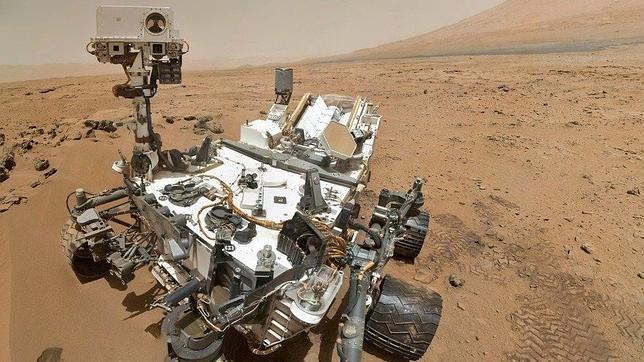
\includegraphics[scale=0.41]{./Figuras/curiosity_marte.jpg}}\hspace{10mm}
\subfigure[Teleoperaci�n m�dica]{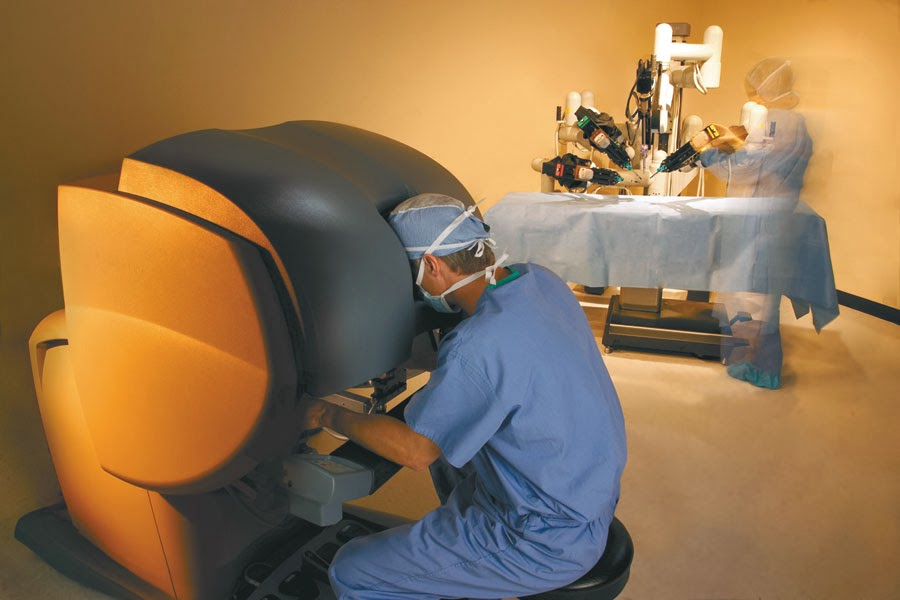
\includegraphics[scale=0.2]{./Figuras/teleoperacion.jpg}}
\caption{Ejemplos de robots}
\label{FIG:1_robotica}
\end{figure}

\subsection{Historia}\label{SEC:Historia}

El origen etimol�gico del t�rmino \textit{robot}, com�nmente utilizado hoy en d�a, tiene como origen la obra con t�tulo \textit{R.U.R}, que es la abreviatura de Rossum's Universal Robots. El escritor de origen checoeslovaco, Karel Capek, invent� la palabra \textit{robota}(labor,trabajo) y cuya ra�z eslava \textit{rabu} coincide con esclavo. La palabra robot a difundida gracias a numerosos autores de �xito en norteamerica, como por ejemplo Isaac Asimov.

Aunque el origen de los robots es anterior a �sta novela de ciencia ficci�n de los a�os 20. Sus predecesores son los aut�matas. La palabra \textit{aut�mata}, de origen griego, se utiliza seg�n la \textit{Real Academia Espa�ola} (RAE) \textit{ para designar a un instrumento o aparato que encierra dentro de s� el mecanismo que le imprime determinados movimientos}. Son artefactos, creados por el hombre, capaces de realizar tareas diarias y comunes para los hombres, o bien, para facilitar las labores cotidianas. Aunque no todos ten�an una utilidad, algunas de ellos serv�an para entretener a sus due�os.

Un ejemplo es el \textit{hombre de palo}(1500) para el emperador Carlos V en Espa�a. Juanelo Turriano construy�  este aut�mata con forma de monje. Andaba y mov�a la cabeza,ojos, boca y brazos. Conforme pasaron los siglos, la complejidad mec�nica fue aumentando hasta llegar por ejemplo, al aut�mata de Maillardet(1800) en Londres. Con una memoria muy superior a cualquier m�quina de la �poca, era capaz de dibujar cuatro dibujos y  escribir tres poemas (dos en franc�s y uno en ingl�s) en un papel.

\begin{figure}[hbtp]
\centering
\subfigure[Aut�mata]{\includegraphics[scale=0.035]{./Figuras/MAILLARDET2.jpg}}
\subfigure[Dibujo en papel]{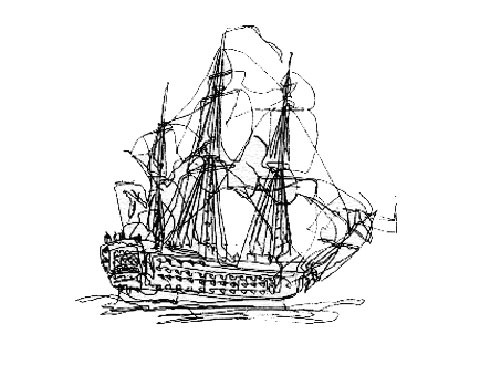
\includegraphics[scale=0.46]{./Figuras/MAILLARDET1.jpg}}
\caption{Aut�mata de Maillardet}
\label{FIG:2_historia1}
\end{figure}

Entre los a�os 1960 y 1980, la aparici�n de los primeros ordenadores revolucionan los aut�matas, llegando por primera vez la rob�tica a las universidades. Un ejemplo es el Stanford Cart. Se utiliz� para demostrar que no se pod�a controlar de forma fiable un veh�culo no tripulado en la Luna. Utilizaba cuatro ruedas con motores el�ctricos y una c�mara. La siguiente evoluci�n de este carrito fue con el logro del primer robot con ruedas y visi�n aut�nomo. Hasta que en 1980, utilizando dos c�maras, se comienza a reconstruir el espacio en 3D mediante la construcci�n de mapas.

\begin{figure}[hbtp]
\centering
\subfigure[Stanford Cart]{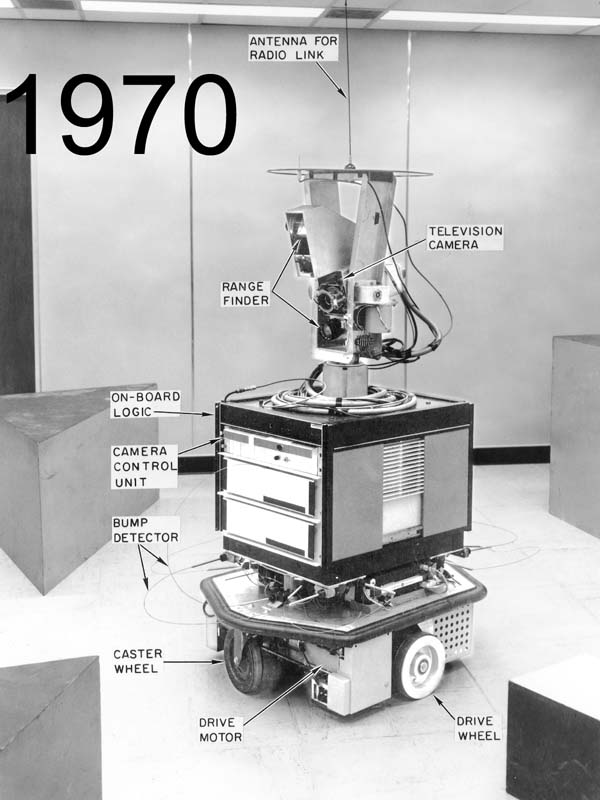
\includegraphics[scale=0.14]{./Figuras/stanford_cart1.jpg}}\hspace{10mm}
\subfigure[Reconstrucci�n del espacio 3D en mapas]{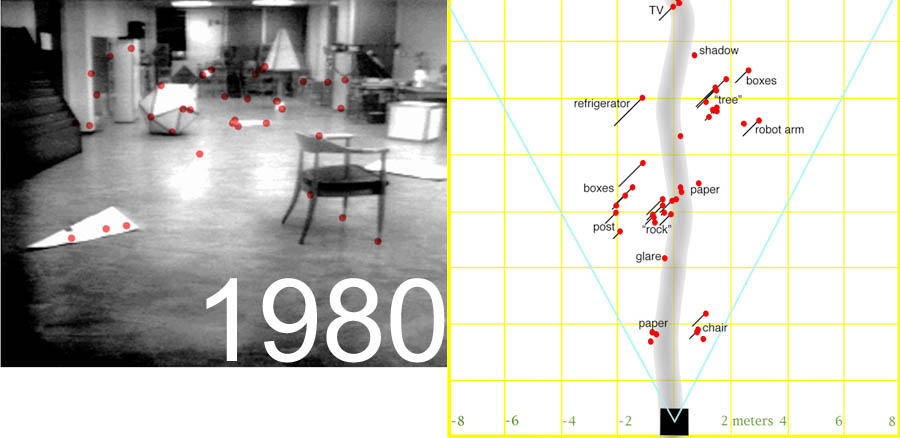
\includegraphics[scale=0.50]{./Figuras/stanford_cart2.jpg}}
\caption{Robot de Stanford Cart}

\label{FIG:3_historia1}
\end{figure}

M�s adelante, con la aparici�n de nuevos sistemas operativos y ordenadores mucho m�s potentes, las aplicaciones de la rob�tica son cada vez m�s extensas y se populariza la interacci�n entre robots y humanos. La compa��a de juguetes LEGO lanza MINDSTORMS. Consist�a en un equipo de desarrollo para robots, basado en piezas de LEGO como estructura y compuesto por un procesador y varios sensores y actuadores. Por otro lado, Sony pone al mercado el primer Aibo, el perro robot. Un juguete pensado para interaccionar con ni�os y simular el comportamiento de una mascota. Los humanoides tambi�n se popularizan como por ejemplo ASIMO. Este robot es presentado por primera vez en el a�o 2000 por la empresa japonesa Honda. Es una demostraci�n del potencial de la rob�tica y un escap�rate para el mundo de lo que se puede hacer. Actualmente sigue sirviendo como exhibici�n de la tecnolog�a empleada por Honda y es capaz de acciones como dar la mano a otra persona, subir escaleras y coger un vaso de agua sin romperlo, entre muchas otras.

\begin{figure}[hbtp]
\centering
\subfigure[LEGO Mindstorms]{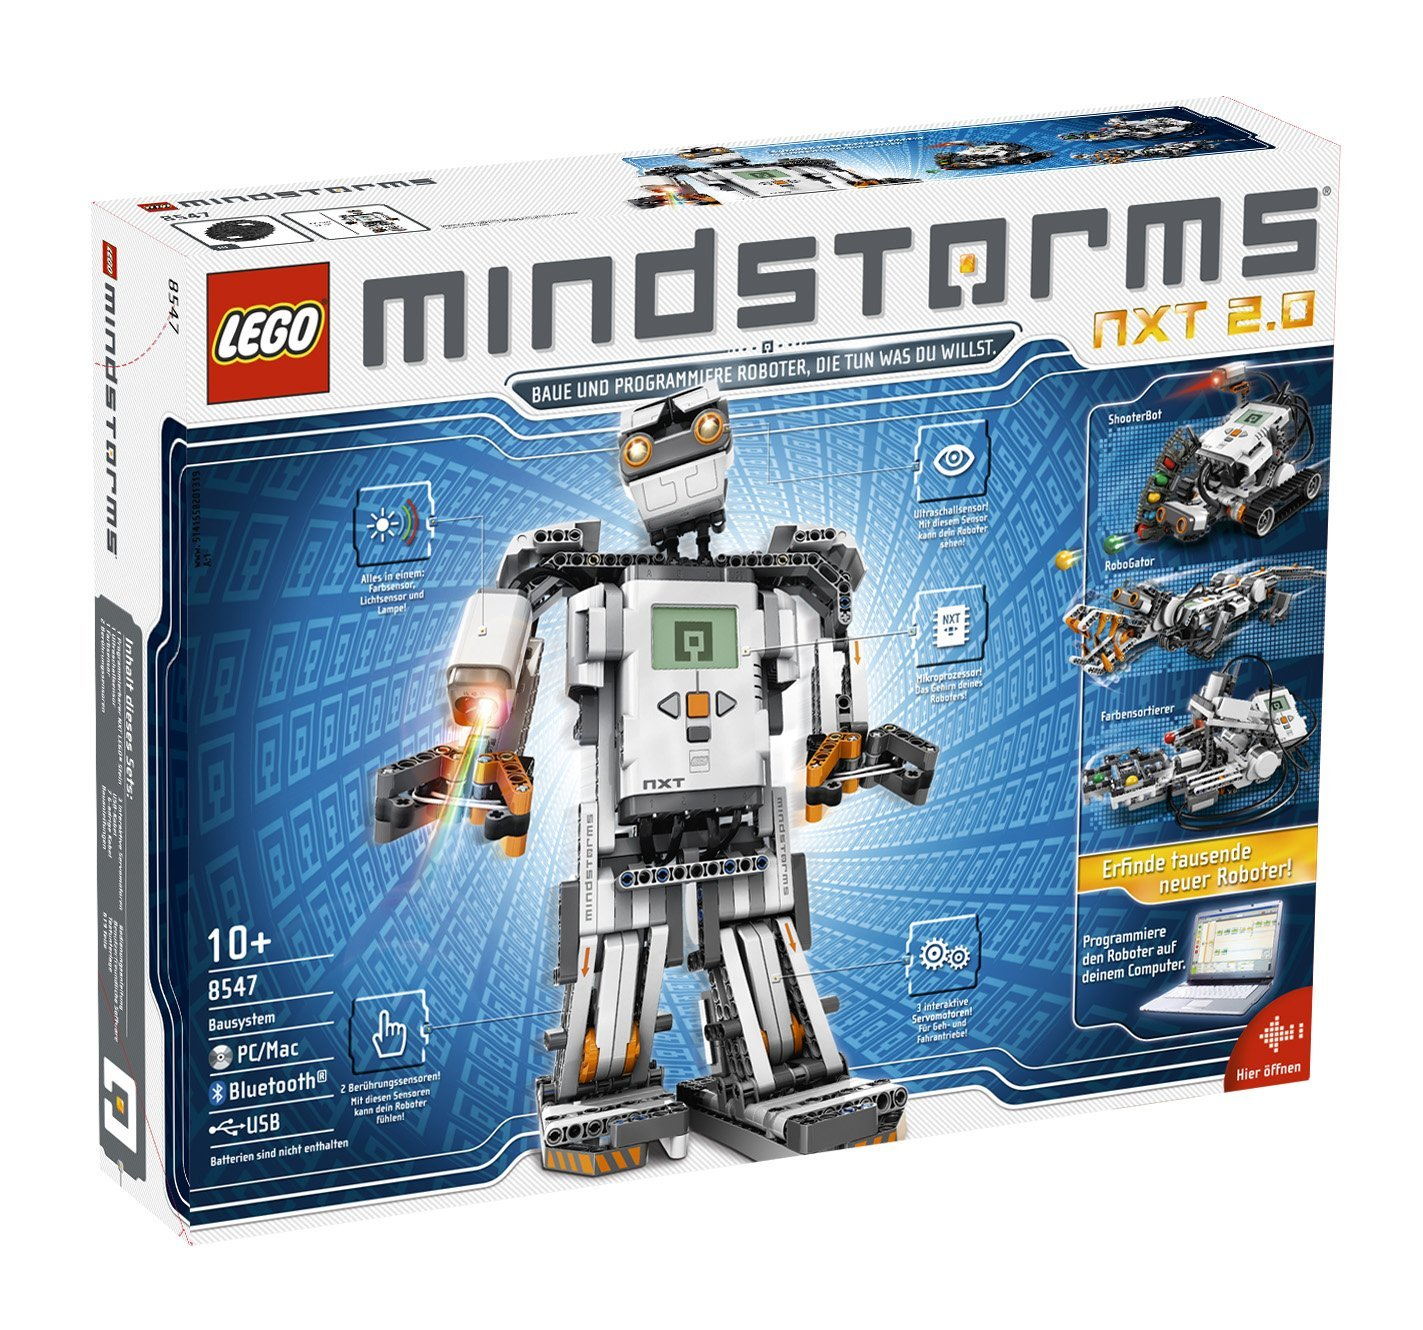
\includegraphics[scale=0.08]{./Figuras/mindstorms.jpg}}\hspace{5mm}
\subfigure[Evoluci�n de Asimo]{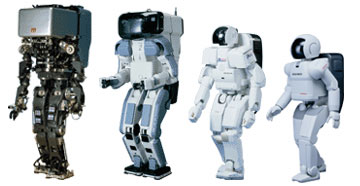
\includegraphics[scale=0.35]{./Figuras/asimo.jpg}}\hspace{5mm}
\subfigure[Aibo]{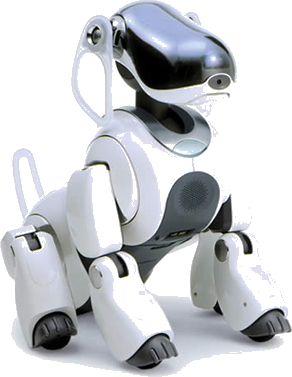
\includegraphics[scale=0.19]{./Figuras/aibo.png}}
\caption{Robots en el siglo XX}
\label{FIG:4_historia1}
\end{figure}

\subsection{Aplicaciones actuales}\label{SEC:Aplic_actual}

Hoy en d�a, las aplicaciones de los robots son muy diversas. Fuera y dentro de nuestro planeta, los robots permiten hacernos ver sitios en los que el hombre no puede llegar o en los que el h�bitat es h�stil. Como el Global Explorer ROV, que se ha sumergido en diferentes oc�anos para obtener im�genes nunca antes vistas por el hombre.

%las aplicaciones de los robots son muy diversas como el uso l�dico, espacial, seguridad, sustituci�n de tareas repetitivas, ayuda e interacci�n social con personas, etc. Robots como Roomba del fabricante iRobot o el AR.Drone de Parrot han acercado la rob�tica a los hogares de muchas personas, siendo su uso f�cil y accesible, incluso si no se tiene conocimiento alguno en este �mbito. 

\subsubsection{Sector industrial}

Es uno de los sectores que m�s compra robots y se encuentra en constante crecimiento. China est� a punto de pasar a EEUU en densidad de robots por trabajador y en Espa�a el uso de robots en empresas aument� un 38\% en 2013\footnote[1]{Datos obtenidos de International Federation of Robotics http://www.ifr.org/}\label{FN:IFR}.

Dentro de las aplicaciones encontramos:

\begin{itemize}
\item Operaciones de manipulaci�n: Usan pinzas, colaboran con otros robots y/u operarios y desplazan objetos. Este uso es uno de los m�s extendidos en empresas. Por ejemplo en el montaje de coches, ayudando a operarios a desplazar objetos pesados como las puertas.
\item Soldadores. Se encargan de las tareas de soldadura de componentes. La compa��a Asus ha creado un m�todo de producci�n autom�tico para sus tarjetas gr�ficas. En concreto, este proceso de soldadura mejora la calidad del producto y permite reducir el tama�o de sus tarjetas notablemente.\footnote{ Introducing ASUS Auto-Extreme Technology: \url{https://www.youtube.com/watch?v=4gRpuurPsuc}}
\item Montaje. Las cadenas de montaje se vuelven m�s r�pidas y eficientes. En las plantas de procesadores Intel, el proceso de montaje es uno de los m�s avanzados del mundo y se utilizan salas en las que el aire no es respirable para personas y garantizan un �rea de part�culas externas muy baja, muy importante para la pureza de los procesadores.
\end{itemize}

\subsubsection{Aplicaciones comerciales}

Su uso est� en constante crecimiento y el n�mero de aplicaciones es muy variado, desde recreaci�n pasando por la grabaci�n profesional para cine. A continuaci�n, se recogen algunas de las aplicaciones que tienen lugar en la actualidad:

\begin{itemize}
\item Limpieza dom�stica: Incluye robots que limpian piscinas, hasta aspiradoras inteligentes. Este �ltima caso es el de Roomba(Figura \ref{FIG:1_Aplicaciones}), de la compa��a iRobot, que incorpora algoritmos de construcci�n de mapas, evasi�n de objetos o incluso detecci�n de escaleras (para evitar posibles accidentes).

\item Transporte de personas:El mayor representante de este tipo de productos es el Google Car(Figura \ref{FIG:1_Aplicaciones}). Este proyecto, en funcionamiento desde 2009, ofrece a personas con movilidad reducida o discapacitados, la utilizaci�n de autom�viles, en concreto un coche. Est� equipado con todo tipo de sensores que permiten la autolocalizaci�n, evitar accidentes y llegar al destino deseado. Dota de mayor autonom�a a estas personas, mejorando su calidad de vida.

\item Seguridad y automatizaci�n en veh�culos: En esta categor�a se recogen sistemas de seguridad que controlan la distancia de seguridad respecto de otros veh�culos, luces inteligentes e incluso sistema de aparcamiento asistido. Compa��as como BMW, Honda o Mercedes Benz apuestan cada d�a m�s por la utilizaci�n de estas tecnolog�as en la industria de automoci�n.

\item Grabaci�n a�rea: La utilizaci�n de drones con la capacidad de volar, ha reducido considerablemente el coste de planos a�reos y simplificado el equipo necesario. Airdog(Figura \ref{FIG:1_Aplicaciones}) es un proyecto nacido de una camapa�a Kickstarter que permite el seguimiento de actividades deportivas o recreativas a gran velocidad, de forma totalmente aut�noma, y la grabaci�n de las mismas.

\end{itemize}

\begin{figure}[hbtp]
\centering
\subfigure[Roomba]{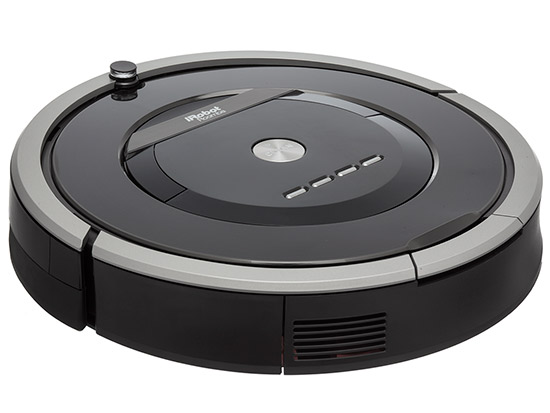
\includegraphics[scale=0.22]{./Figuras/roomba.jpg}}\hspace{5mm}
\subfigure[Google Car]{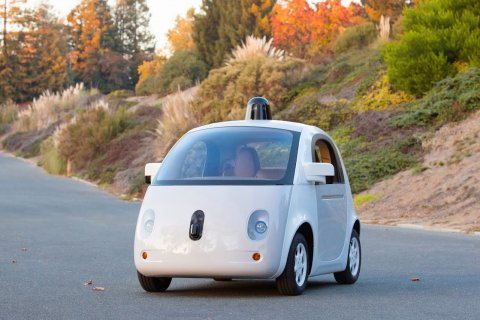
\includegraphics[scale=0.235]{./Figuras/google-selfdrivingcar.jpg}}\hspace{5mm}
\subfigure[Secuencia de seguimiento de un Airdog]{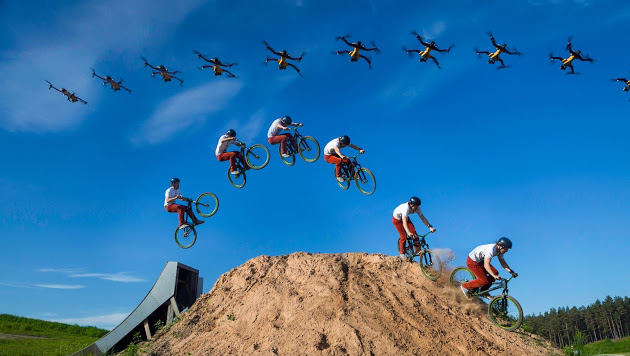
\includegraphics[scale=0.21]{./Figuras/air_dog.jpg}}\hspace{5mm}
\caption{Aplicaciones en la actualidad}
\label{FIG:1_Aplicaciones}
\end{figure}

\subsection{Software en robots}\label{SEC:Software en robots}

El software que se encuentra en los robots, es el encargado de dotar de un comportamiento inteligente a los mismos. Se pueden distinguir tres tipos software en un robot. Uno, es el sistema operativo que se ocupa del procesador. El segundo es el que se encarga, por ejemplo, de calcular el movimiento necesario de cada actuador bas�ndose en algoritmos. Se caracteriza porque puede contener diferentes niveles de lenguaje. Desde unos de alto nivel, como el que utilizar�a cualquier programa que ejecuta en un ordenador, hasta otros de bajo nivel, como el c�digo m�quina. El �ltimo grupo es la colecci�n de programas y funciones desarrolladas para utilizar los perif�ricos del robot. Dicha colecci�n, abstrae los dos grupos anteriormente explicados en beneficio de una programaci�n m�s f�cil.

\section{Visi�n en robots}\label{SEC:Visi�n artificial en robots}
La visi�n, al igual que en los seres humanos, es una gran fuente de informaci�n de nuestro entorno. Las personas utilizamos el espectro visible de la luz, que se corresponde con lo que llamamos colores. Adem�s, percibimos el mundo que nos rodea como un mundo en tres dimensiones debido a que tenemos dos ojos. Esto nos permite obtener propiedades del entorno y poder  desplazarnos en �l sin preocupaciones. Los robots utilizan sensores de visi�n de todo tipo, capaces de ver en la oscuridad o distinguir diferentes temperaturas. Adem�s, en los �ltimos a�os, los sensores de visi�n han disminu�do en precio y su utilizaci�n se ha visto incrementada notablemente en el mundo de la rob�tica. A pesar de este incremento en su uso y de ser una fuente potencialmente rica en informaci�n, el flujo de datos puede llegar a ser muy grande y su procesado complicado.

El objetivo de la visi�n artificial es conseguir datos a trav�s de las im�genes que recibe de una c�mara. Para esto se aplican diferentes operaciones matem�ticas con el fin de conseguir bordes, formas, colores, patrones en la imagen, etc�tera. 

\subsection{Aplicaciones actuales}

Actualmente, las aplicaciones de visi�n artificial son muy variadas, desde seguridad, como sistemas de detecci�n de movimiento, pasando por el entretenimiento, como el sensor Kinect, hasta la accesibilidad para dotar de autonom�a a personas que lo necesitan. Es muy com�n, hoy en d�a, que un robot incluya como parte de sus sensores una c�mara. 

\begin{itemize}
\item Navegaci�n y construcci�n de mapas: Es una de las primeras aplicaciones a trav�s de visi�n y permite a los robots la creaci�n de mapas a trav�s de la detecci�n de bordes, formas o profundidad. �sta informaci�n sirve tambi�n para poder navegar sobre sitios desconocidos o previamente han sido convertidos a un mapa. Un ejemplo hoy en d�a el \textit{Darpa Robotics Challenge}\footnote{Web oficial de Darpa Robotics Challenge \url{http://www.theroboticschallenge.org/}}, en el que la visi�n es un elemento crucial para poder esquivar objetos y realizar mapas del terreno.
\item Autolocalizaci�n: Permite extraer informaci�n a un robot sobre la posici�n relativa respecto al resto del mundo que lo rodea, mediante el reconocimiento de patrones o balizas. Una t�cnica es el SLAM (\textit{Simultaneous Localization and Mapping}), que permite la autolocalizaci�n al mismo tiempo que se realiza un mapa del entorno. 

\end{itemize}


\begin{figure}[hbtp]
\centering
\subfigure[Reconocimiento de objetos en imagen]{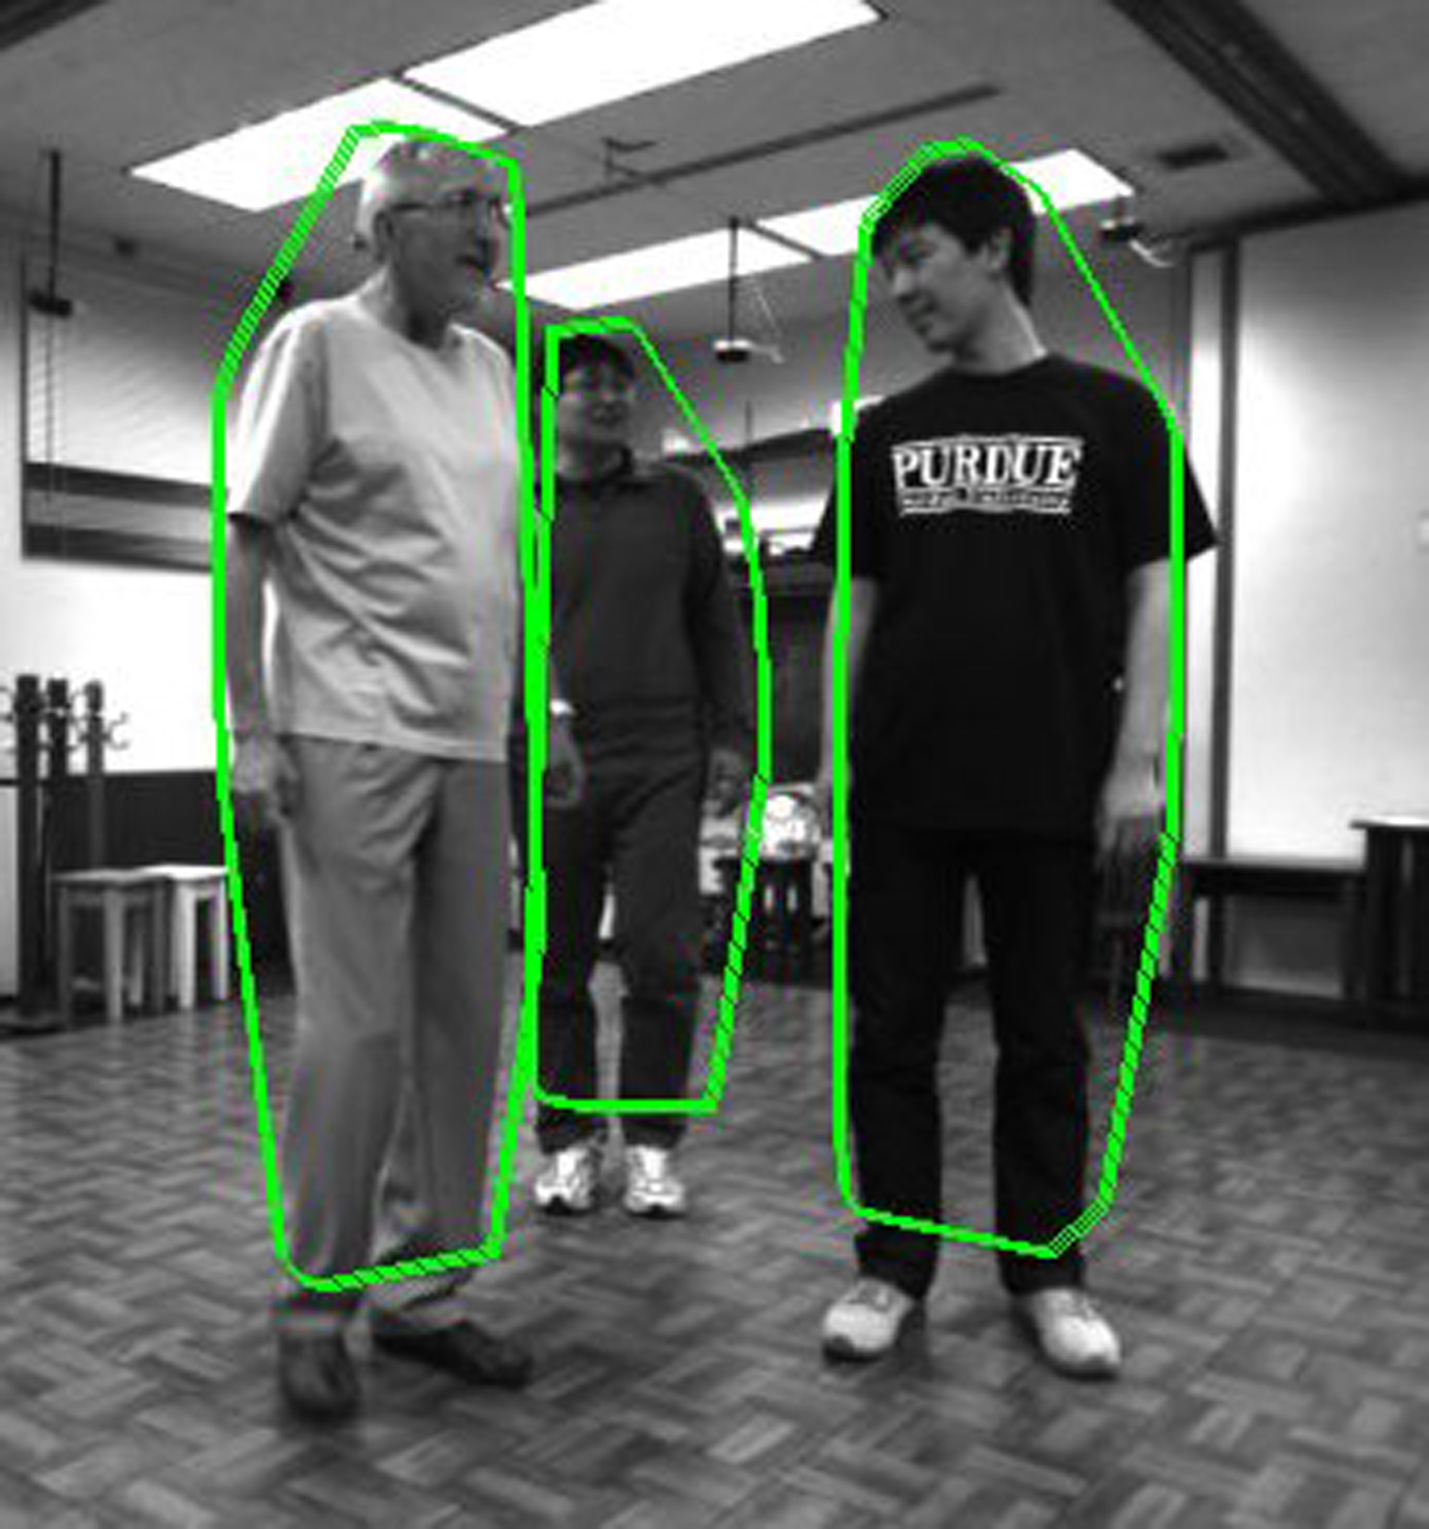
\includegraphics[scale=0.08]{./Figuras/robotic_vision1.jpg}}\hspace{10mm}
\subfigure[Reconstrucci�n de mapas con t�cnicas SLAM]{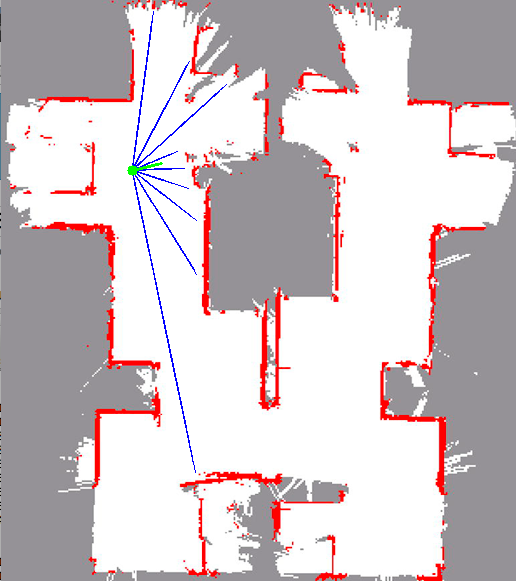
\includegraphics[scale=0.21]{./Figuras/SLAM.png}}
\caption{Visi�n artificial en robots}

\label{FIG:5_vision}
\end{figure}



\section{Simulaci�n}\label{SEC:Simulaci�n}

Una parte importante del dise�o del comportamiento de un robot, es la simulaci�n. Proporciona un entorno virtual en el que somete a diferentes escenarios y situaciones a un modelo creado a partir del robot elegido. Permite probar algoritmos sin necesidad de utilizar uno real.  Puede llegar a aportar informaci�n muy valiosa y familiarizarse con posibles situaciones. Adem�s de prevenir accidentes como cualquier da�o f�sico al objeto o herir a las personas cercanas. El problema que se presenta es que los resultados dependen de la precisi�n a la hora de caracterizar el modelo y mundo virtual. Una vez alcanzado el resultado deseado, se ha de adaptar nuestra aplicaci�n rob�tica al mundo real. 

Son necesarios motores de f�sica como Bullet, que simplifican el c�lculo y la representaci�n de f�sicas reales en tiempo real para la interacci�n entre objetos. 

Todo esto no ser�a posible sin un motor gr�fico, que dibuje en pantalla todo lo que est� ocurriendo. Se ocupan de dar realismo y representar en im�genes el mundo virtual con el que estamos trabajando. Un ejemplo es Ogre u OpenGL, que dan una gran variedad de opciones, como la renderizaci�n de texturas y sombras.

Para una mayor precisi�n del comportamiento en el mundo real, los simuladores incluyen la adici�n de funciones de ruido en sensores y actuadores. Esto permite la creaci�n de comportamientos mucho m�s robustos.

Un ejemplo es Gazebo\footnote{P�gina web oficial de Gazebo : \url{http://gazebosim.org/}}, un proyecto de software libre que incluye multitud de modelos y motores de f�sica virtualizada. Ofrece una interfaz gr�fica y control sobre los objetos y el mundo generado, adem�s de la creaci�n y modificaci�n de actuadores y sensores personalizados. Por ejemplo, se pueden crear veh�culos con diferentes sensores o casas con las que interactuar.

\begin{figure}[hbtp]
\centering
{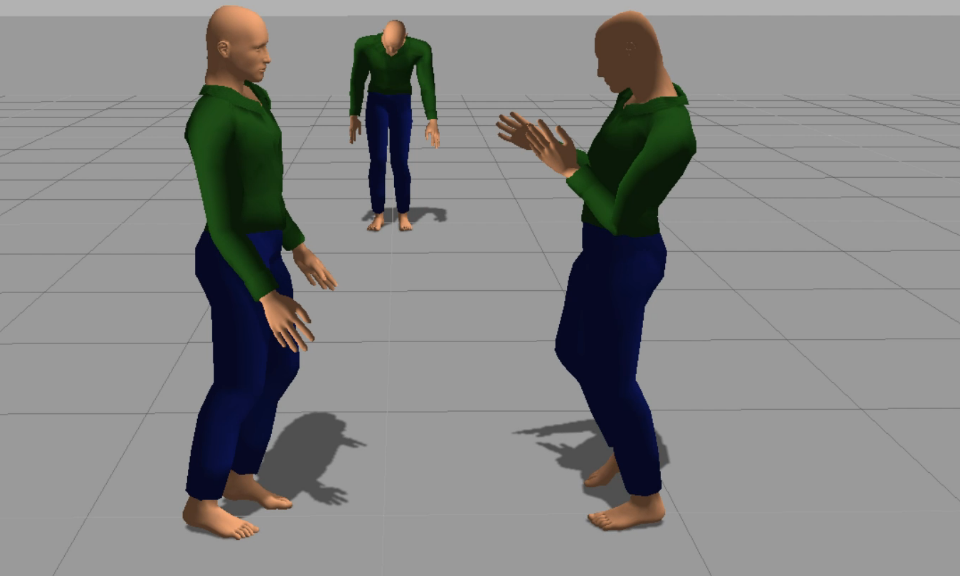
\includegraphics[scale=0.3]{./Figuras/gazebo2.png}}\hspace{10mm}
%\subfigure[Personas en Gazebo]{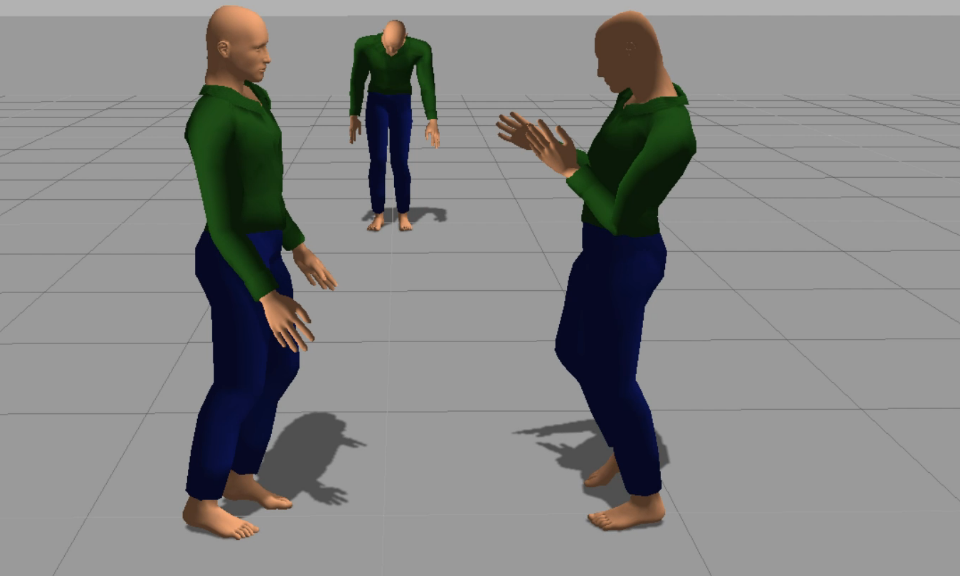
\includegraphics[scale=0.26]{./Figuras/gazebo2.png}}
\caption{Personas simuladas en Gazebo}

\label{FIG:6_simulacion}
\end{figure}

El desarrolo de Gazebo comenz� en 2002 en la Universidad de California del Sur por Andrew Howard y Nate Koenig. A partir del concepto de un simulador de alta precisi�n para poder simular robots en entornos exteriores bajo diferentes circunstancias. El nombre elegido fue Gazebo ya que es la estructura m�s cercana a un escenario de exteriores. 

A pesar del origen de este nombre, hoy en d�a se utiliza para la simulaci�n de interiores tambi�n. Es uno de los componentes oficiales en \textit{Virtual Robotics Challenge} organizado por \textit{DARPA Robotics Challenge}(DRC). Actualmente su desarrollo se encuentra bajo el \textit{Open Source Robotics Foundation}(OSRF) con soporte de una variada y activa comunidad. Por �ltimo, es utilizado como herramienta de virtualizaci�n oficial para la plataforma \textit{JdeRobot} de la Universidad Rey Juan Carlos.

\begin{figure}[hbtp]
\centering
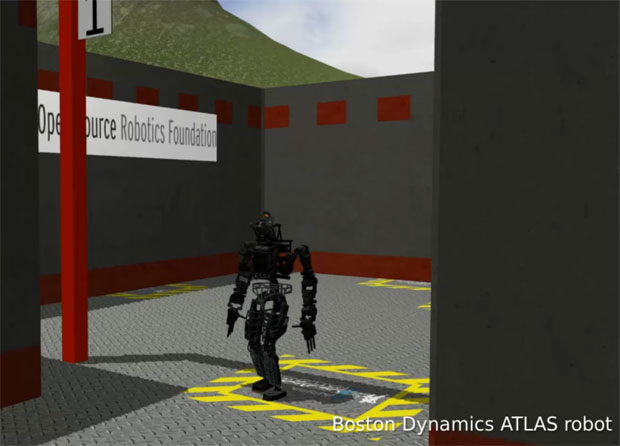
\includegraphics[scale=0.4]{./Figuras/DRCChallenge.jpg}
\caption{Robot utilizado en DRC}
\label{FIG:7_simulacion}
\end{figure}

\section{Rob�tica A�rea}\label{SEC:Rob�tica A�rea}

Es una de las ramas de la rob�tica de mayor auge actualmente y sus aplicaciones son cada vez m�s extendidas. Pertenecen a este �rea los \textit{Unmanned Aircraft Vehicle}(UAV),en espa�ol \textit{Veh�culo A�reo No Tripulado}(VANT), o tambi�n conocidos como \textit{drones}. Se trata de un veh�culo capaz de volar, que puede o no recibir �rdenes del exterior. Incluyen multitud de diferentes sensores para mantenerse en vuelo, aterrizar o despegar.

\subsection{Historia}

Hist�ricamente, el origen de los \textit{UAV} ha sido en aplicaciones militares, como en otras �reas de investigaci�n. Una vez ha sido suficientemente desarrollado comienzan las aplicaciones civiles y su aplicaci�n comercial e industrial.
En 1883, Douglas Archibald instal� un anem�metro, un instrumento para medir la velocidad del viento, a su cometa para poder medir la velocidad del viento a una altura de m�s de 350 metros. En 1887 instal� dos c�maras, de las cuales tom� fotograf�as una vez en el aire. Se consideran las primeras im�genes tomadas por un \textit{UAV}. M�s tarde se usar�a esta t�cnica en la guerra entre Espa�a y los Estados Unidos en 1898 para obtener datos estrat�gicos.

%Durante la Primera Guerra Mundial, se utilizaron \textit{UAV} cargados con explosivos que era llevado por un avi�n y se soltaba para realizar el ataque. M�s tarde, en 1924, Montgomery Low consigui� eleminir las interferencias que produc�a el motor de los \textit{UAV} y establecer una conexi�n para conseguir el primer vuelo controlado a trav�s de radio.
Durante la primera y la segunda guerra mundial se utilizaron drones para la obtenci�n de mapas sin poner en peligro al piloto. M�s tarde, en 1995 se utilizaron en Bosnia para tareas de vigilancia o an�lisis de da�os. Especialmente importante para el reonocimiento nocturno. El modelo se llamaba \textit{Predator} y era lanzado desde Hungr�a.

\begin{figure}[hbtp]
\centering
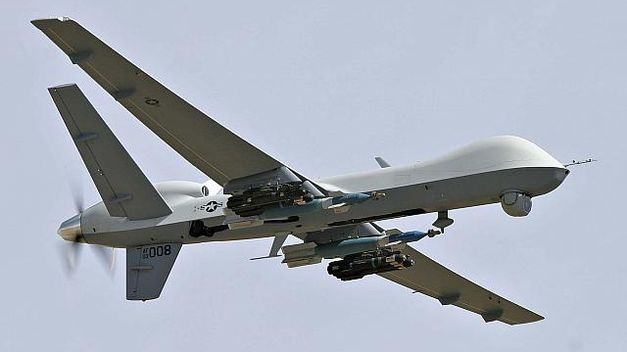
\includegraphics[scale=0.25]{./Figuras/predator.jpg}
\caption{UAV Predator.}

\label{FIG:8_historia2}
\end{figure}

\subsubsection{Aplicaciones actuales}

Actualmente, gracias al avance de la estabilizaci�n electr�nica, los \textit{UAV} han alcanzado tama�os mucho m�s reducidos, como el \textit{Hummingbird}\footnote{M�s informaci�n en: \url{http://www.avinc.com/nano}} o colibr� en espa�ol, de \textit{DARPA}. Adem�s son mucho m�s �giles y mec�nicamente simples. Han aparecido numerosos usos comerciales y civiles, aunque no desaparece el inter�s militar. Compa��as como \textit{Amazon}, est�n trabajando en proyectos para conseguir crear un sistema de env�o de compra a domicilio utilizando \textit{drones}, en concreto \textit{cuadric�pteros}. En universidades como \textit{University of Pennsylvania} est�n dise�ando comportamientos basados en grupos masivos, creando formaciones en el aire y dotando capacidad de pensamiento en grupo a los drones. Otro de los usos es la exploraci�n a�rea, que incluye la inspecci�n de embalses, l�neas de alta tensi�n, campos agr�colas y la vigilancia. Este �ltimo caso es el de Alemania, que utiliza drones aer�os para evitar el ataque de grafiteros a vagones de tren\footnote{Alemania pone a prueba drones contra los grafitis: \url{http://www.bbc.com/mundo/noticias/2013/05/130528_tecnologia_drones_graffiti_alemania_aa}}.
Uno de los campeonatos m�s recientes de programaci�n para \textit{UAV} es el \textit{Mohamed Bin Zayed International Robotics Challenge}(MBZIRC)\footnote{P�gina Web oficial del campeonato: \url{http://www.mbzirc.com/}}. Con una recompensa de 5 millones de d�llares, una de las pruebas consiste en localizar, seguir y aterrizar, coincidiciendo con los objetivos principales de este Trabajo Fin de Grado.

\begin{figure}[hbtp]
\centering
\subfigure[Amazon Prime]{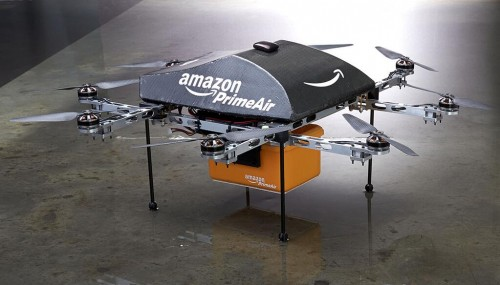
\includegraphics[scale=0.35]{./Figuras/amazon_prime.jpeg}}\hspace{5mm}
\subfigure[Grupos masivos]{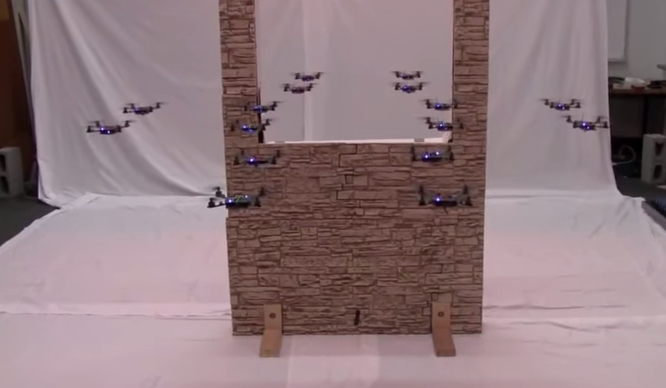
\includegraphics[scale=0.26]{./Figuras/xhover.png}}
\caption{Ejemplos de UAV civiles}

\label{FIG:9_historia2}
\end{figure}

\subsubsection{Cuadric�pteros}

Existen diferentes tipos de \textit{drones} en funci�n del dise�o y los componentes que los forman. Algunos son similares a los aviones, con alas y el mismo m�todo de despegue y aterrizaje. Est�n pensandos para largos per�odos de tiempo y altas velocidades.
Otros, buscan una excepcional maniobrabilidad y estabilidad a�rea. En este caso utilizan rotores, al igual que los helic�pteros. A este grupo pertenecen los \textit{cuadric�pteros}. Se caracterizan por ser un helic�tpero multi-rotor de cuatro brazos en forma de cruz. Los rotores, se encuentran en el extremo de cada brazo. 

Cuando los motores giran, las h�lices situadas en ellos generan un fuerza de empuje vertical, llamada \textit{sustentaci�n}. �sta es perpendicular al movimiento de la h�lice y depende de la velocidad a la que gira. La suma de cada fuerza en cada rotor produce una resultante. Los diferentes movimientos que puede describir el cuadric�ptero se encuentran recogidos en la ilustraci�n de la Figura\ref{FIG:10_historia2}. El color rojo indica que una potencia mayor ha sido aplicada, mientras que el verde, respresenta una potencia menor. Para evitar un fen�meno que en los helic�pteros produce vueltas sobre s� mismo, la disposici�n de los motores sigue una forma de cruz, en la que cada par opuesto gira en el mismo sentido. Uno en el sentido de las agujas del reloj y el otro anti-horario.

Para que sea posible el despegue (Figura\ref{FIG:10_historia2},e), esta resultante ha de ser superior al peso del \textit{UAV}. Si es igual, se consigue un estado de altitud fija (tambi�n conocida en ingl�s como \textit{hovering}). Para aterrizar ser�a necesario una resultante menor que el peso del objeto (Figura\ref{FIG:10_historia2},f).

Para conseguir el giro conocido como \textit{yaw} (Figura\ref{FIG:10_historia2},g y h) o \textit{gui�ada}, es el giro del plano horizontal al \textit{drone}. Para girar a la derecha se transmite m�s potencia al par de rotores que giran en sentido anti-horario. Si la potencia fuera superior en el otro par opuesto, giraria hacia la izquierda sobre s� mismo.

En el supuesto de que s�lo uno de los motores aplicase m�s potencia que los dem�s, por ejemplo el delantero, el \textit{cuadric�ptero} se deplazar�a hacia atr�s, inclinando la parte trasera del veh�culo hacia arriba. Esto se corresponder�a con el movimiento llamado \textit{pitch}(Figura\ref{FIG:10_historia2},a y b) o \textit{cabeceo}.

Por �ltimo, si aumentamos la potencia en uno de los motores laterales, por ejemplo la derecha, el veh�culo se inclinar� y trasladar� hacia la izquierda, provocando un movimiento conocido como \textit{roll}(Figura\ref{FIG:10_historia2},c y d) o \textit{alabeo}. 

\begin{figure}[hbtp]
\centering
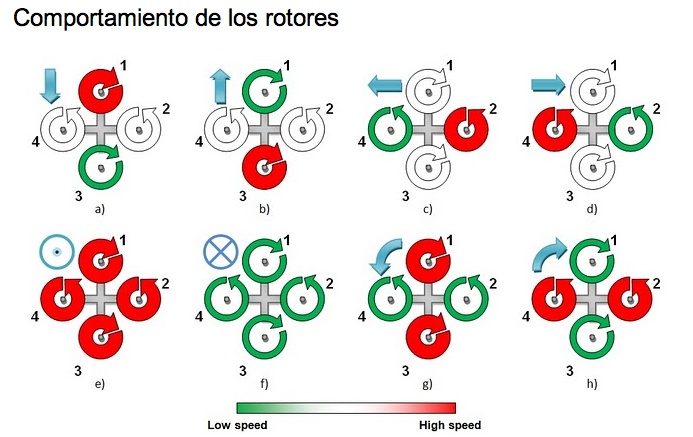
\includegraphics[scale=0.6]{./Figuras/rotores.png}
\caption{Relaci�n entre la potencia de los rotores y el movimiento de un cuadric�ptero}
\label{FIG:10_historia2}
\end{figure}
Los cuadric�pteros pueden tener numerosos sensores desde aceler�metros, giroscopios, magnet�metros, ultrasonidos, incluso c�maras con resoluciones de hasta 4K. Todo ello se utiliza en combinaci�n, para conseguir una mayor estabilizaci�n durante el vuelo. Dentro de los actuadores encontramos los cuatro rotores pero tambi�n se pueden a�adir pinzas para cargar objetos o, en caso de uso militar, armas y sus respectivos gatillos.

Algunos de los fabricantes de drones m�s relevantes actualmente son:

\begin{itemize}
\item Parrot: Con modelos como el Ar.Drone 1 y 2 que acercaron a un gran p�blico el uso de los drones.
\item 3DRobotics: Dise�ado para la obtenci�n de planos a�reos 
estables.
\item  Erle: Est� soportado oficialmente por Ubuntu.
\item Airdog: Ya mencionado previamente en el apartado \ref{AIRDOG}
\end{itemize}

\subsection{Rob�tica A�rea en la Universidad Rey Juan Carlos}

El grupo de Rob�tica de la Universidad Rey Juan Carlos lleva a�os desarrollando proyectos relacionados con la navegaci�n, visi�n, autolocalizaci�n y virtualizaci�n de entornos con robots. Gracias a la popularizaci�n y a la reducci�n en coste de los \textit{drones} se comenz� en el a�o 2013 una nueva l�nea de investigaci�n sobre los \textit{UAV}. Los primeros proyectos han creado las bases sobre las que seguir investigando y han proporcionado la infraestructura necesaria. �stos han sido integrados en la plataforma JdeRobot, en la cual participan profesores, alumnos y gente de la comunidad de software libre. Sirve como base para nuevos proyectos o la mejora de los actuales. Recientemente ha formado parte de el \textit{Google Summer of Code 2015} en el que personas de todo el mundo, ofrecen su colaboraci�n para mejorar un proyecto de software libre.

Entre estos proyectos se encuentra el Trabajo de Fin de Grado(TFG) \textit{Navegaci�n visual en robots a�reos} de Alberto Mart�n. Sus aportaciones a JdeRobot fueron la de un componente llamado \textit{ardrone\_server}, que crea una interfaz capaz de comunicarse con el \textit{AR.Drone} de la compa��a \textit{Parrot}. En el mismo trabajo, incluye una herramienta, llamada \textit{uav\_viewer} cuya funci�n es obtener la informaci�n de los sensores y controlar los actuadores de dicho \textit{UAV}. Por �ltimo, se encuentra un componente de visi�n y navegaci�n llamado \textit{object\_tracking}. Utiliza filtros de colores para el seguimiento de objetos a trav�s de las im�genes recibidas por la c�mara frontal y ventral del \textit{drone}. El drone es  capaz de un seguimiento aut�nomo de objetos, tanto en el suelo como en 3D.

\begin{figure}[hbtp]
\centering
\subfigure[ArDrone sin y con protecci�n de interiores]{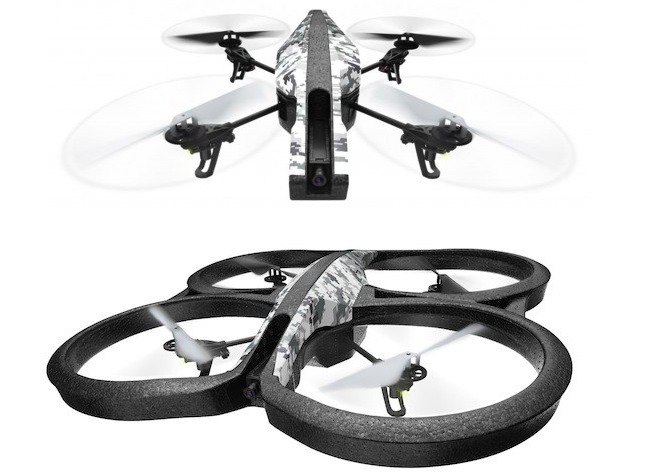
\includegraphics[scale=0.28]{./Figuras/ardrone.jpg}}\hspace{3mm}
\subfigure[Interfaz gr�fica del componente uav\_viewer]{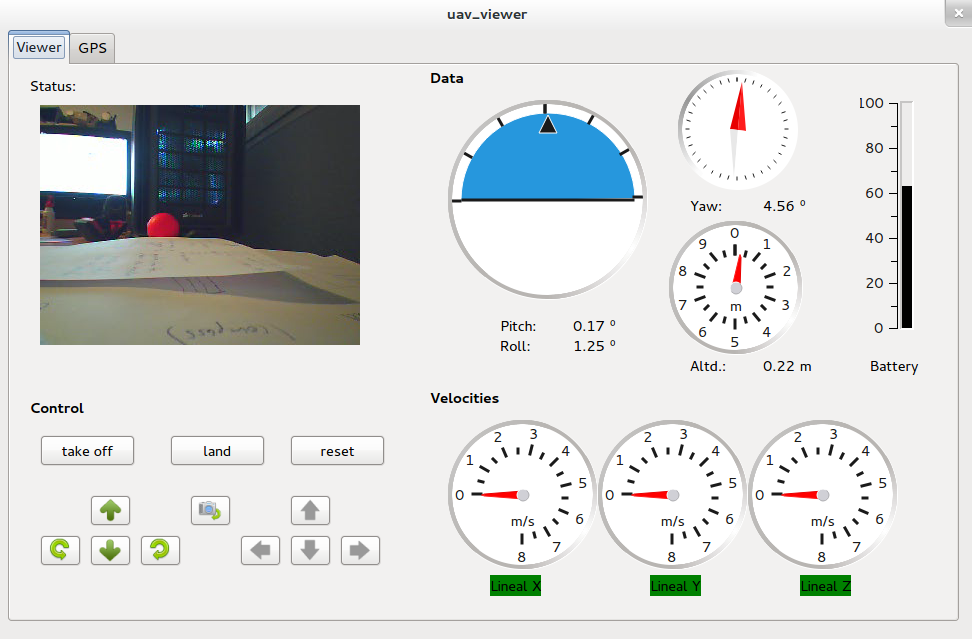
\includegraphics[scale=0.22]{./Figuras/uav_viewer.png}}
\caption{Simulaci�n en exteriores}

\label{FIG:11_urjc}
\end{figure}

Daniel Yag�e en su Proyecto Fin de Carrera \textit{Cuadric�ptero AR.Drone en Gazebo y JdeRobot}, desarroll� un modelo para la plataforma \textit{JdeRobot} en el simulador \textit{Gazebo} del mismo \textit{AR.drone} que utiliz� Alberto Mart�n, anteriormente mencionado. Esto permite tanto la simulaci�n de los datos sensoriales como de la virtualizaci�n realista de un comportamiento cercano a dicho \textit{drone}. Adicionalmente, program� diferentes aplicaciones de navegaci�n aut�nomas como el seguimiento de balizas por posici�n, seguimiento de carretera o el seguimiento de otro cuadric�ptero. Para ello, crea unas interfaces inclu�das en el entorno de \textit{JdeRobot} que permiten el desarrollo de otras aplicaciones de navegaci�n. 

\begin{figure}[hbtp]
\centering
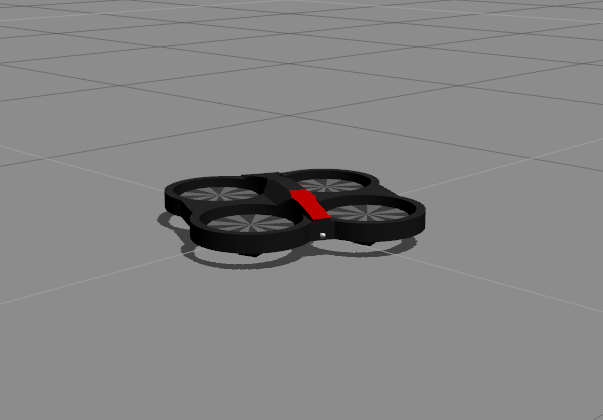
\includegraphics[scale=0.4]{./Figuras/ArDrone_model.png}
\caption{ArDrone simulado en Gazebo}

\label{FIG:12_urjc}
\end{figure}

Siguiendo con las bases aportadas por los dos proyectos previamente explicados, en este TFG se programar� el comportamiento aut�nomo de aterrizaje de un drone sobre una baliza visual, m�vil o est�tica. Se utilizar� un drone simulado en Gazebo, empleando la infraestructura existente en JdeRobot para estos cuadric�pteros. Con ello se pretende dar un salto adelante a�adiendo un nuevo comportamiento a los ya disponibles.

%se aplicar�n los conceptos explicados en este cap�tulo. Se aplicar� el sistema de visualizaci�n \textit{April Tags} y se generar�n todos los componentes necesarios para crear un entorno virtualizado en el que poder observar los resultados obtenidos.

En el pr�ximo cap�tulo, se explicar�n los objetivos y la m�todolog�a propuesta para resolverlos. En el tercer cap�tulo se expondr�n con profundidad la infraestructura y herramientas  utilizadas. En el cuarto, se describir� el desarrollo de todos los componentes que forman este proyecto. En quinto lugar, se realizar�n distintos experimentos para observar los datos obtenidos en diferentes escenarios y validar experimentalmente la soluci�n programada. Para terminar, unas conclusiones aportar�n un visi�n global del conjunto y los conocimientos extra�dos.


\newpage \thispagestyle{empty} \cleardoublepage
\chapter{Objetivos}\label{CAP:Objetivos}

\section{Tareas que cumplir}

El objetivo principal de este Trabajo de Fin de Grado es desarrollar una aplicaci�n, que a trav�s de la aplicaci�n de una t�cnica de visi�n artificial, dote de un comportamiento aut�nomo a un \textit{drone} en el que busque una baliza visual y aterrice sobre ella. Para llegar a �l, ha sido fundamental dividir el proyecto en objetivos m�s peque�os, que sumados, dan forma a todo el conjunto. 

 \begin{itemize}
 
 \item Dise�o de un coche y desarrollo de un plugin, ambos para Gazebo, con una baliza visual en su techo.
 
 \item Dise�o y desarrollo una aplicaci�n de control visual para la localizaci�n, seguimiento y aterrizaje en un objeto preparado para la tarea. Se compone de una parte perceptiva, que recoge la informaci�n de las im�genes, y una parte de control y actuaci�n, que generar� los diferentes comportamientos del cuadric�ptero.
 
 \item Validaci�n experimental en el cuadric�ptero simulado. Se realizar�n varias pruebas para demostrar el correcto funcionamiento de la infraestructura y del control visual.
  
 \end{itemize}

\section{Requisitos}

Se deber�n satisfacer, adicionalmente, los siguientes requisitos:

\begin{itemize}

\item Los componentes y aplicaciones desarrollados han de estar integrados en la plataforma \textit{JdeRobot}.

\item El control del cuadric�ptero simulado ha de ser flu�do, de modo que pueda seguir objetos en movimiento a 5 cm/seg.

\item Los componentes y aplicaciones desarrollados han de ser computacionalmente eficientes.

\end{itemize}

\section{Metodolog�a}

Para poder materializar los objetivos y requisitos, previamente mencionados, es necesario aplicar alg�n m�todo que defina las distintas etapas y estados. En este Trabajo de Fin de Grado se aplica el m�todo de dessarrollo en espiral. Este modelo, creado por Barry Boehm en 1986, se utiliza frecuentemente en la ingenier�a de software. Se basa en una serie de iteraciones en bucle. En cada ciclo, se realiza un conjunto de cuatro actividades:

\begin{enumerate}
\item \textbf{Determinar los objetivos}: Poner limitaciones definidas en forma de objetivos o resquisitos. Dividir el proyecto en partes m�s peque�as.
\item \textbf{An�lisis del riesgo}: Estudiar los riesgos de cada uno de los objetivos que se abordan. Evaluar las alternativas posibles en caso de amenazas.
\item \textbf{Desarrolar y probar}: Verificaci�n de la tarea actual. Al mismo tiempo, se realiza un an�lisis para encontrar nuevos factores de riesgo, como errores que se podr�an arrastran a la pr�xima iteraci�n.
\item \textbf{Planificaci�n}: Establecer y definir las fases anteriores.
\end{enumerate}

\begin{figure}[h]
 \centering
 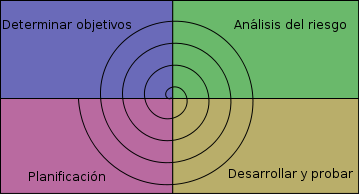
\includegraphics[width=90mm]{Figuras/desarrollo_en_espiral.png}
 \caption{Representaci�n del desarrollo en espiral.}
 \label{fig:21_planificacion_espiral}
\end{figure}

\section{Planificaci�n}

Durante el desarrolo de este proyecto, se han establecido reuniones peri�dicas con el tutor. En ellas, revis�bamos los objetivos anteriormente fijados y los resultados obtenidos. Si alguno de los objetivos generaba alg�n problema o no se llegaba al resultado deseado, se aplazaban o se profundizaba en la ra�z del problema. A continuaci�n, se determinaban los subobjetivos de nuestro pr�ximo encuentro. 

Como parte de la evaluaci�n de los objetivos propuestos, ha sido fundamental la utilizaci�n del \textit{mediawiki}\footnote{http://jderobot.org/Andresjhe-tfg}  de la plataforma \textit{JdeRobot}. En el publicaba, a modo de cuaderno de bit�cora, redactando los �xitos y progresos, haciendo uso adem�s de contenido multimedia como im�genes o v�deos. 

Para el seguimiento y almacenamiento del software desarrolado hemos empleado la herramienta Subversion. Todo el c�digo relacionado con este proyecto se encuentra alojado en mi repositorio\footnote{https://svn.jderobot.org/users/andresjhe/tfg}.



\begin{itemize}

\item Familiarizaci�n con el entorno de \textit{JdeRobot}: Incluye el estudio de las dependencias necesarias para la instalaci�n del entorno. Estudio de las diferentes bibliotecas, interfaces y componentes. Aprendizaje y profundizaci�n de lenguajes de programaci�n como Python y C++, as� como la herramienta para las comunicaciones ICE. As� como el estudio y familiarizaci�n de la biblioteca April Tags para la detecci�n de los mismos y la biblioteca de visi�n OpenCV. 

\item Familiarizaci�n con Gazebo. Se ha estudiado los plugins ya existentes en JdeRobot y a su vez, la creaci�n otros nuevos a trav�s de la API de Gazebo. El aprendizaje de Blender ha sido necesario para generar el modelo virtual de un veh�culo. Por �ltimo, se ha desarrolado su respectivo plugin en Python para teledirigir y asignar rutas al veh�culo anteriormente generado. Se ha desarrollado un componente integrado en JdeRobot que calcule y dibuje distancias a partir de la posici�n  de modelos en el simulador Gazebo.

\item Estudio del dispositivo MK802IV para una modificaci�n del software para ser empleado como unidad de procesamiento junto al AR.Drone. Adicionalmente, se ha investigado diferentes medios para realizar la comunicaci�n con el drone.

\item Desarrollo de la aplicaci�n que se encarga del control visual. En este punto se han creado diferentes mundos en Gazebo y se han dise�ado distintos comportamientos en el veh�culo.

\item Validaci�n experimental, en la que se validar� en funci�n de los resultados la soluci�n programada.

\end{itemize}


\newpage \thispagestyle{empty} \cleardoublepage
\chapter{Infraestructura}\label{CAP:MatMet}

 En cada uno de los siguientes apartados se detallar� la funci�n de los programas o dispositivos necesarios para la elaboraci�n de este proyecto.
 Debido a la naturaleza de la plataforma JdeRobot, el sistema operativo que se ha elegido para el desarrollo y ejecuci�n de los componentes ha sido Linux. En concreto, la distribuci�n Ubuntu 14.04.

\section{Interfaz Gr�fica de usuario}
Tambi�n conocida como \textit{GUI}, es el software encargado de simplificar la interacci�n con los usuarios. Proporciona texto, im�genes y diferentes objetos gr�ficos para representar la informaci�n y e interactuar con las acciones que se ofrezcan en un programa.

\subsection{Qt}
Qt\footnote{http://www.qt.io/} es una biblioteca multiplatarforma cuyo objetivo principal es el de facilitar el dise�o de interfaces gr�ficas de usuario. Su modelo de desarrollo es el de software libre y de c�digo abierto, bajo la licencia GPL v3 y LGPL v2.1. Est� programada en C++, aunque puede ser utilizada junto a otros lenguajes de programaci�n. Ofrece un \textit{ambiente de desarrollo integrado}(IDE en ingl�s) llamado QtCreator, que facilita el proceso de desarrollo y el dise�o gr�fico del GUI. La versi�n utilizada en este proyecto es la 4.8.

\begin{figure}[hbtp]
\centering
{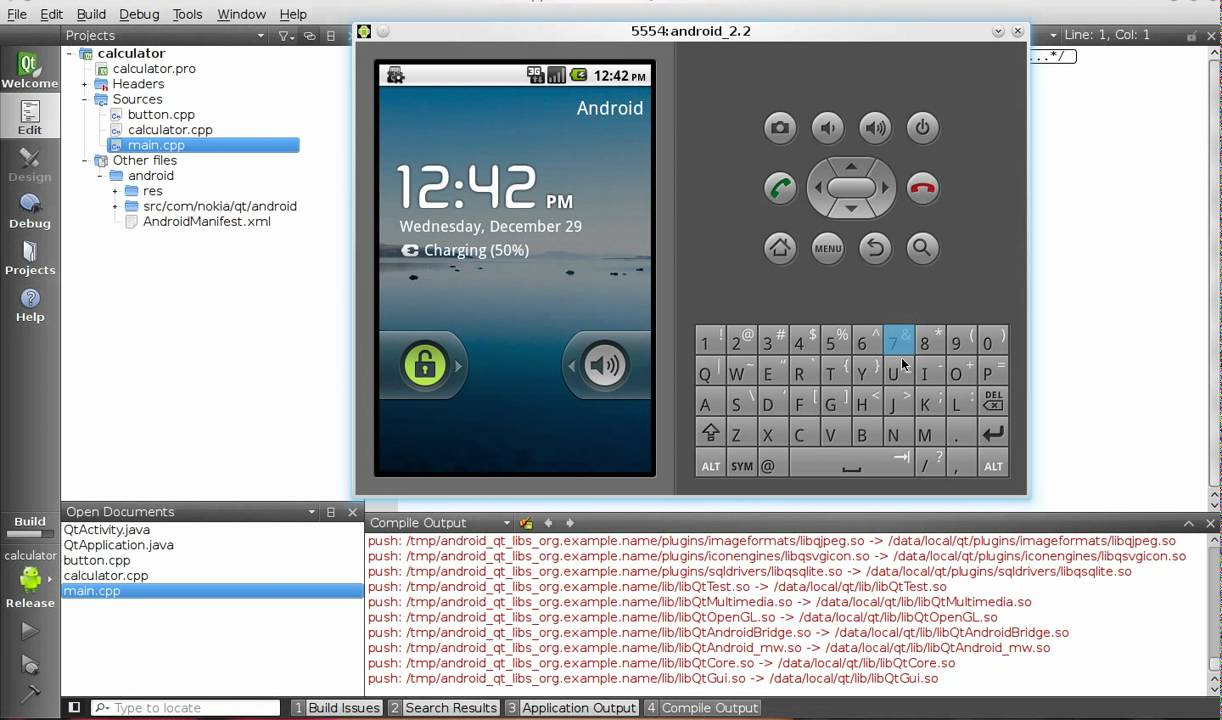
\includegraphics[scale=0.2]{./Figuras/qt.jpg}}\hspace{10mm}
%\subfigure[Personas en Gazebo]{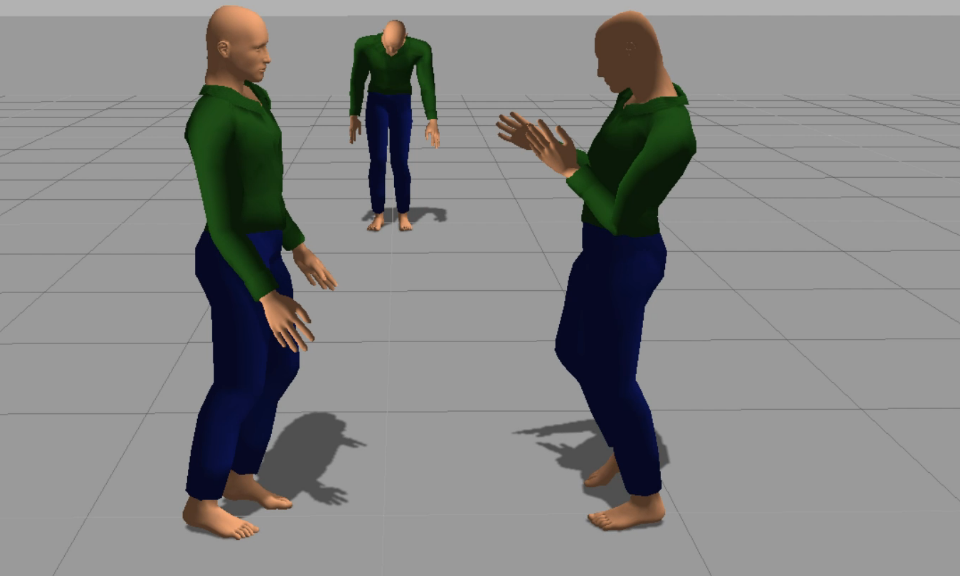
\includegraphics[scale=0.26]{./Figuras/gazebo2.png}}
\caption{Qt Creator}

\label{FIG:31_qtcreator}
\end{figure}

\subsubsection{PyQt}

PyQt\footnote{https://riverbankcomputing.com/software/pyqt/intro} es una colecci�n de bibliotecas escritas en Python y C++ que complementan Qt. Mantiene la caracter�stica multiplataforma  y es un partner reconocido oficialmente por el propio Qt. Se encuentra bajo la licencia GPL v3 y la \textit{Riverbank Commercial License}. En este proyecto se ha utilizado para el desarrollo de componentes utilizando el lenguaje de programaci�n Python. La versi�n utilziada en este proyecto es la PyQt5.

\subsection{Matplotlib}

Matplotlib\footnote{http://matplotlib.org/} es una librer�a en python para dibujar gr�ficas en dos dimensiones. Ofrece una interfaz muy cercana a la ofrecida por el programa \textit{Matlab} y su utilizaci�n resulta muy familiar para usuarios que dominan este programa. Su principal ventaja es la simplicaci�n a la hora de dibujar diferentes estilos de l�neas, cambiar las propiedades de ejes, las propiedades del texto, etc�tera.


\section{ICE}

ICE\footnote{https://zeroc.com/} es un middleware orientado a objetos proporciona las herramientas, APIs y librer�as necesar�as para simplificar las comunicaciones entre cliente y servidor. En JdeRobot es la plataforma elegida como infraestructura para todos los procesos de comunicaci�n entre componentes y plugins. Proporciona una capa transparente que se encarga de abrir y cerrar conexiones, la serializaci�n de informaci�n, retransmisi�n de paquetes perdidos, etc�tera. La versi�n utilizada en este proyecto es la 3.5

\section{JdeRobot}

En el mundo de la rob�tica, existen diferentes plataformas que simplifican y aportan las herramientas necesarios para el desarrollo de aplicaciones en robots. JdeRobot es una de ellas y consiste en una colecci�n de aplicaciones rob�ticas, dom�ticas y de visi�n artificial. Estas aplicaciones est�n escritas en diferentes lenguajes como C++, Java o Python y su interoperaci�n se realiza a trav�s de interfaces ICE. En ella participan desarrolladores de diferentes niveles desde profesionales del sector, profesores, alumnos de la Universidad Rey Juan Carlos y de otras universidades de todo el mundo. 
Durante el ciclo de vida este proyecto ha servido como plataforma de exposici�n de los progresos y logros conseguidos. El c�digo fuente es libre y est� bajo la licencia GPLv3 y la documentaci�n se encuentra protegido bajo la licencia de Creative Commons by-SA.

Durante el desarrollo de este TFG, comoponentes como uav\_viewer, introrob\_py han servido de referencia y han tenido una gran relevancia para el aprendizaje de la plataforma.
La versi�n utilizada en este proyecto es la 5.2.4\footnote{https://github.com/RoboticsURJC/JdeRobot}

\subsection{Teleoperadores uav\_viewer e introrob\_py}

Ambos son componentes de JdeRobot y su funci�n es la de ofrecer una GUI para enviar comandos tanto al cuadric�ptero real, como al Ardrone creado por Daniel Yag�e. 
Los comandos se env�an a trav�s de interfaces ICE. Estos permiten el desarrollo de programas independientemente del tipo de cuadric�ptero(real o simulado) y transportan la informaci�n de los sensores. La principal diferencia entre ambos es el lenguaje en el que han sido desarrollados: introrob\_py est� escrito en Python mientras que uav\_viewer est� en C++.

\begin{figure}[hbtp]
\centering
{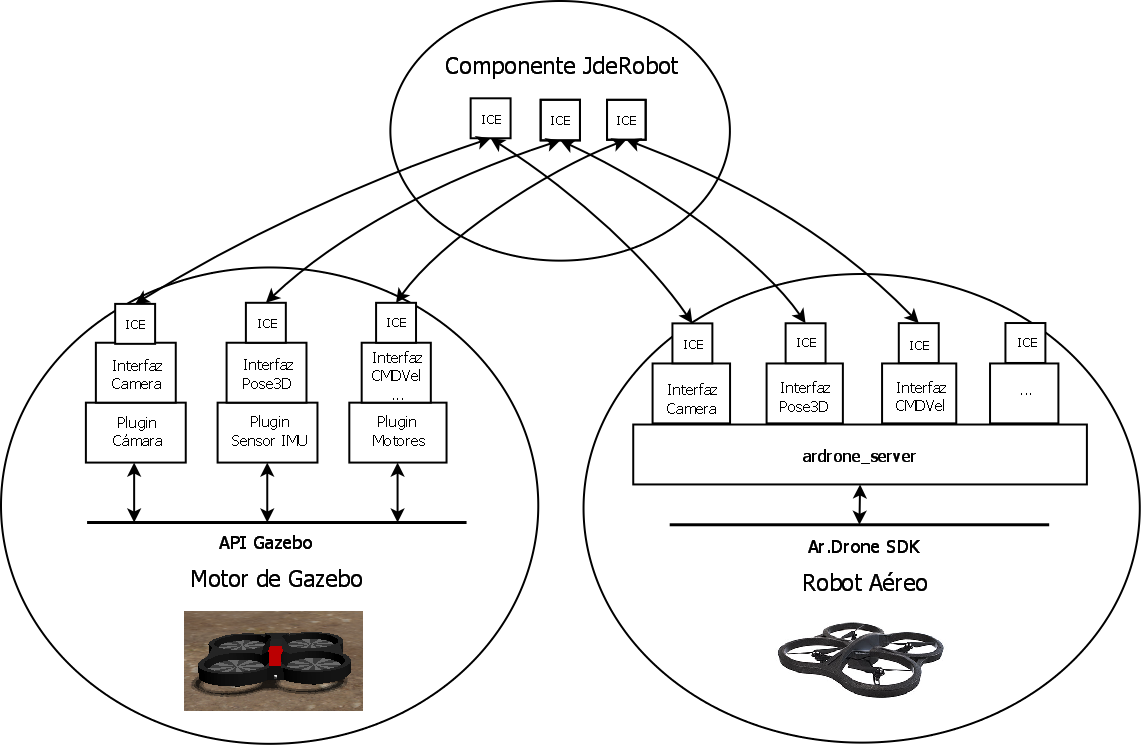
\includegraphics[scale=0.28]{./Figuras/ardroneplugin-connections.png}}
\caption{Interfaz de JdeRobot para el AR.Drone}

\label{FIG:32_JdeRobot}
\end{figure}

\section{Gazebo}

La herramienta en la que se realizan todas las pruebas es el entorno de simulaci�n Gazebo. Ya fue introducido en el apartado \ref{SEC:Simulaci�n}, por tanto, hablaremos de su estructura y las bibliotecas de las que se sirve este proyecto.

Gazebo se divide en dos programas:

\begin{enumerate}
\item \textbf{Gzclient}: Es la GUI a trav�s la cual visualizar los resultados y comportamientos de nuestros modelos virtuales. Ofrece diferentes herramientas como la pausa de la simulaci�n, toma de instant�neas, a�adir objetos sobre la marcha, etc�tera.

\item \textbf{Gzserver}: Este programa se encarga del control de la simulaci�n, la generaci�n del mundo virtual y el motor f�sico.
\end{enumerate}

La estructura que define una simulaci�n en Gazebo se compone de varios elementos:

\begin{itemize}
\item \textbf{Mundos}: Describen todos los elementos que contiene una simulaci�n, incluyendo robots, luces, sensores y objetos est�ticos. Est�n escritos en formato SDF (explicado m�s adelante) y usan la extensi�n \textit{.world} .

\item \textbf{Modelos}: Se generan a partir de archivos en formato SDF. Contienen las propiedades y los plugins necesarios para la simulaci�n. Gazebo incluye una base datos de robots que se descarga a trav�s de Internet. Estos modelos pueden ser insertados y facilitan la familiarizaci�n con el entorno.

\item \textbf{Variables de entorno}: Se utiliza para localizar los diferentes archivos como mundos, modelos o plugins.

\item \textbf{Plugins}: Son un mecanismo para interacci�n con Gazebo a trav�s de su API\footnote{http://gazebosim.org/api.html}. Permiten la modificaci�n de par�metros durante la simulaci�n, con el fin de cambiar el comportamiento de los modelos. 

\end{itemize}

\subsubsection{Formato SDF}
Algunos de los elementos anteriormente mencionados utilizan el formato SDF, el cual se basa en lenguaje XML para describir las propiedades de los mundos y modelos en Gazebo.
\begin{figure}[hbtp]
\centering
{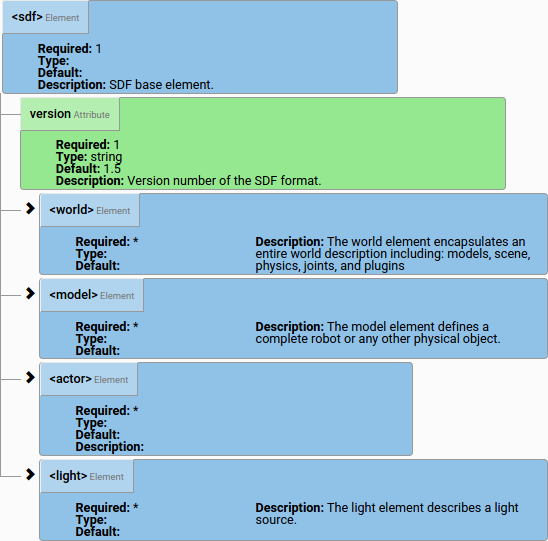
\includegraphics[scale=0.55]{./Figuras/sdf.png}}
%\subfigure[Personas en Gazebo]{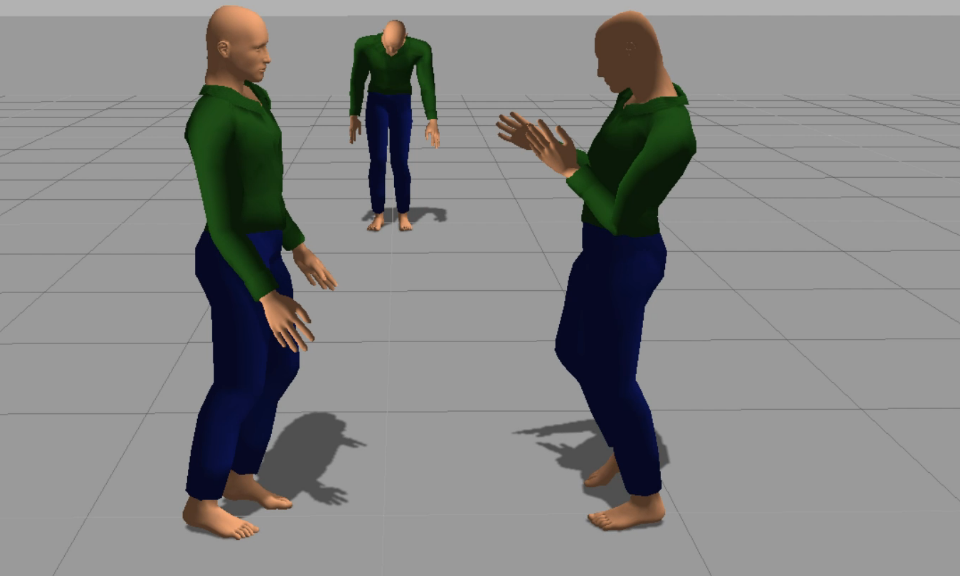
\includegraphics[scale=0.26]{./Figuras/gazebo2.png}}
\caption{Ejemplo del formato SDF}

\label{FIG:32_sdf}
\end{figure}

\subsection{Plugins}

Los plugins permiten acceder a todas las funcionalidades de Gazebo a trav�s de clases en C++ descritas en la su respectiva API\footnote{http://gazebosim.org/api.html}. 

\section{Blender}

\section{Visualizaci�n virtual}

\subsection{AprilTags}

En este proyecto, se utilizar� una librer�a basada en visualizaci�n virtual denominada \textit{AprilTags}. Es un sistema de visualizaci�n fiduciaria. Estos sistemas se basan es s�mbolos dise�ados para ser f�cilmente reconocidos del resto del entorno. Puede detectar uno o varios s�mbolos en la misma imagen. Adem�s de proporcionar informaci�n como la identificaci�n y posici�n del s�mbolo dentro de una imagen. Es un sistema robusto cuyo funcionamiento es independiente del �ngulo y diferentes sistuaciones de luminosidad en la imagen.

\begin{figure}[hbtp]
\centering
{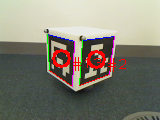
\includegraphics[scale=0.9]{./Figuras/apriltag.png}}
%\subfigure[Personas en Gazebo]{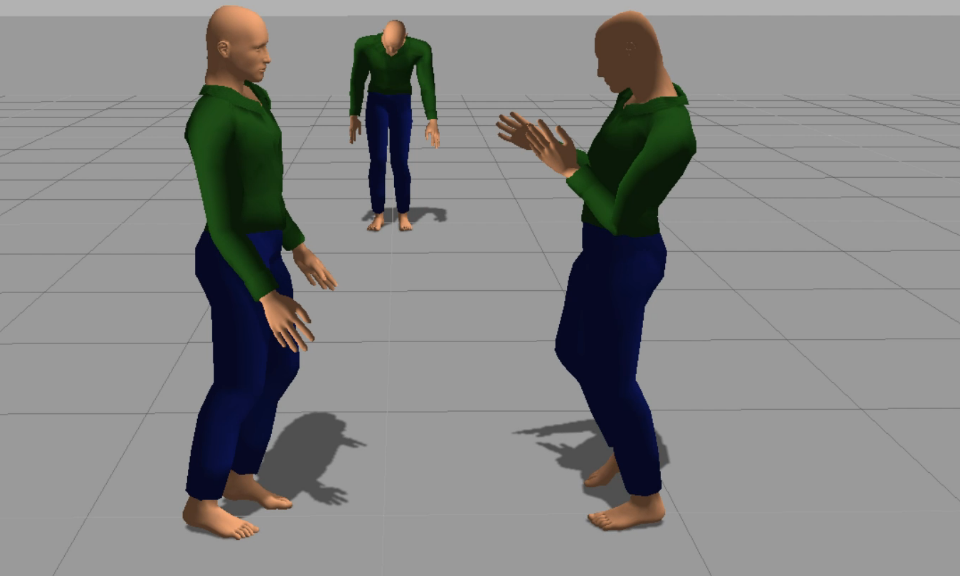
\includegraphics[scale=0.26]{./Figuras/gazebo2.png}}
\caption{Ejemplo de detecci�n en AprilTag}

\label{FIG:33_apriltag}
\end{figure}

Sus aplicaciones son muy variadas, desde la captura de moviento en objetos hasta sistemas de balizas en t�cnicas de navegaci�n. Otra de sus aplicaciones es la de \textit{realidad aumentada}, sustituyendo el s�mbolo por una imagen virtualizada.

Originalmente est� escrita en C y Java pero Ed Olson de Massachusetts Institute of Technology(MIT) ha creado una adaptaci�n en C++. El c�digo\footnote{https://svn.csail.mit.edu/apriltags} es abierto y est� protegido bajo la LGPLv2.1. Entre sus depencias se encuentran OpenCV y Eigen3 que son conocidas bibliotecas de tratamiento de imagen en Linux.

Los s�mbolos se dividen en diferentes familias. Estas familias utilizan un n�mero de bits y de distancia de Hamming diferentes.

\begin{figure}[hbtp]
\centering
{
\includegraphics[scale=0.22]{./Figuras/apriltags-codes.png}}
%\subfigure[Personas en Gazebo]{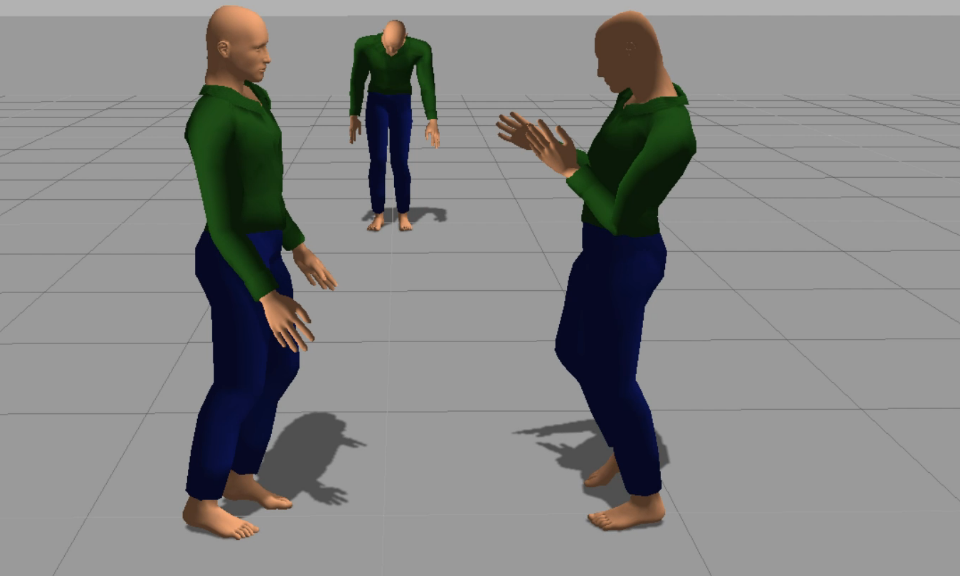
\includegraphics[scale=0.26]{./Figuras/gazebo2.png}}
\caption{Ejemplos de familias en AprilTag}

\label{FIG:34_apriltag_families}
\end{figure}


\subsection{OpenCV}

\section{Dispositivos f�sicos}

\subsection{MK802IV}

\subsection{Ar.Drone 2}



\newpage \thispagestyle{empty} \cleardoublepage
\chapter{Desarrollo de la infraestructura}\label{CAP:Resul}

\section{Coche virtual y teleoperador}

Diana

\section{Mk802IV}

\section{Distance Viewer}
\newpage \thispagestyle{empty} \cleardoublepage
\chapter{Aterrizaje visual}\label{CAP:Aterrizaje visual}


\section{Control visual}


\newpage \thispagestyle{empty} \cleardoublepage
\chapter{Conclusiones y l�neas futuras}\label{CAP:Conclu}
Incluyendo discusi�n de los logros principales alcanzados y posibles trabajos futuros.

\section{Conclusiones}
Bla, bla, bla,...

\subsection{T�tulo de la primera subsecci�n}
Bla, bla, bla,...

\section{L�neas futuras}
Bla, bla, bla,...


\newpage \thispagestyle{empty} \cleardoublepage



%%%%%%%%%%%%%%%%%%%%%%%%%%%%%%%%%%%%%%%%%%%%%%%%%%%%%%%%%%%%%%%%%%%%%%%%
\backmatter
%%%%%%%%%%%%%%%%%%%%%%%%%%%%%%%%%%%%%%%%%%%%%%%%%%%%%%%%%%%%%%%%%%%%%%%%

%\pagenumbering{Roman}%

% BIBLIOGRAF�A _________________________________________________________
\bibliographystyle{./Bibliografia/IEEEtran}
\bibliography{./Bibliografia/RefsPFC}
\addcontentsline{toc}{chapter}{\bibname}
\newpage \thispagestyle{empty} \cleardoublepage
\nocite{*} % [Sin comentar] Incluye todas las referencias, hayan sido citadas o no.

% �NDICE DE TABLAS _____________________________________________________
%\listoftables \addcontentsline{toc}{chapter}{\listtablename}
%\newpage \thispagestyle{empty} \cleardoublepage


%% �NDICE DE ALFAB�TICO ________________________________________________
%{
%\twocolumn \small \setlength{\columnsep}{2cm}
%\printindex \addcontentsline{toc}{chapter}{\indexname}
%}
%\newpage \thispagestyle{empty} \cleardoublepage
%
%\onecolumn


\end{document}



